\documentclass[a4paper]{article}
\usepackage[italian]{babel}
\usepackage[T1]{fontenc}
\usepackage[utf8]{inputenc}
\usepackage{graphicx}
\usepackage[margin=1in]{geometry}
\usepackage{makecell}
%\usepackage[svgnames,table]{xcolor}
\usepackage[table]{xcolor}
% --- Per lo sfondo
%\usepackage{eso-pic,graphicx}
% ---
\usepackage{setspace}

\usepackage{tabularx} 

\usepackage{hyperref}
\usepackage{array}

\usepackage{fancyhdr}

% Definizione comandi personali - Team
\newcommand{\FP}{Francesco Protopapa}
\newcommand{\GC}{Greta Cavedon}
\newcommand{\LW}{Luciano Wu}
\newcommand{\PV}{Pietro Villatora}
\newcommand{\EP}{Edoardo Pavan}
\newcommand{\MG}{Michele Gatto}
\newcommand{\MB}{Matteo Basso}

% Definizione File
\newcommand{\G}{\textit{Glossario v1.0.0}}
\newcommand{\AdR}{\textit{Analisi dei Requisiti v1.0.0}}
\newcommand{\PdP}{\textit{Piano di Progetto v1.0.0}}
\newcommand{\PdQ}{\textit{Piano di Qualifica v1.0.0}}
\newcommand{\SdF}{\textit{Studio di fattibilità v1.0.0}}
\newcommand{\NdP}{\textit{Norme di Progetto v1.0.0}}

% Definizione ruoli
\newcommand{\AN}{Analista}
\newcommand{\VE}{Verificatore}
\newcommand{\AM}{Amministratore}
\newcommand{\RE}{Responsabile}
\newcommand{\PT}{Progettista}
\newcommand{\PR}{Programmatore}

\newcommand{\glo}{\textsuperscript{G}}

%Abbreviaizoni requisiti
\newcommand{\Ob}{Obbligatorio}
\newcommand{\De}{Desiderabile}
\newcommand{\Fa}{Facoltativo}

%Abbrevizioni fonti requisiti
\newcommand{\Di}{Decisione interna}
\newcommand{\Vi}{Verbale interno}
\newcommand{\Ve}{Verbale esterno}
\newcommand{\Ca}{Capitolato}

%link in blu
\newcommand{\mylink}[1]{\color{blue}\url{#1}\color{black}}
\makeindex

\usepackage{hyperref}

\usepackage{longtable}

% Per evidenziare il testo
\usepackage{tcolorbox}




\begin{document}

	% Intro documento 

\begin{center}

\begin{figure}
\centering

\includegraphics[scale=0.05]{Contenuto/Immagini/DreamTeam.png} 
\end{figure}

{\Huge{\textbf{Norme di Progetto}}} \\ [1cm]

\begin{table}[htbp]
\centering
\begin{tabular}{r|c}
\multicolumn{2}{c}{\textbf{Informazioni sul Documento}} \\
\hline \\
\textbf{Versione} & 3.0.0 \\ \rule{0pt}{3ex}    
\textbf{Data di approvazione} & 2022-06-18  \\ \rule{0pt}{2ex} 
\textbf{Approvatori} & \MB{} \\ \rule{0pt}{3ex}      
\textbf{Redattori} & \MG{} \\ \rule{0pt}{2ex}   
& \PV{} \\ \rule{0pt}{3ex}    
\textbf{Verificatori} 
  & \GC{} \\ \rule{0pt}{2ex}
& \EP{} \\ \rule{0pt}{2ex} 
      
\textbf{Uso} & Interno \\ \rule{0pt}{3ex}    
\textbf{Distribuzione} & Prof. Vardanega Tullio \\ \rule{0pt}{2ex}   
& Prof. Cardin Riccardo \\ \rule{0pt}{2ex}   
& Gruppo \textit{DreamTeam} \\ \rule{0pt}{0.1cm}   
\end{tabular} \\ [0.5cm]
\end{table}

\textsl{ e-mail: \href{mailto:dreamteam.unipd@gmail.com}{dreamteam.unipd@gmail.com} } \\[2cm]
\end{center}
\pagebreak	
	% Inserimento di header e footer

\pagestyle{fancy}
\fancyhf{}
\rhead{Analisi dei Requisiti}
\lhead{
\includegraphics[scale=0.015]{Sezioni/images/DreamTeam.png}}
\rfoot{\thepage}
\setlength{\headheight}{35pt}

%\cfoot{Pagina \thepage}
%\setlength{\headheight}{35pt}
%\setcounter{tocdepth}{5}
%\setcounter{secnumdepth}{5}
%\renewcommand{\footrulewidth}{0.4pt}
	% Registro Modifiche

{\LARGE{\textbf{Registro delle Modifiche}}} \\
\begin{table}[!htbp]
\begin{tabular}{|m{0.1\textwidth}<{\centering}|m{0.1\textwidth}<{\centering}|m{0.2\textwidth}<{\centering}|m{0.2\textwidth}<{\centering}|m{0.3\textwidth}<{\centering}|}
	\hline \rowcolor{gray!50}
	\textbf{Versione}&\textbf{Data}&\textbf{Nominativo}&\textbf{Ruolo}&\textbf{Descrizione}\\ 
	\hline
	0.1.0& 06.12.21& \shortstack{ } &\shortstack{ \\ \VE{} } & Verifica del corretto output del documento in latex\\
	\hline
	0.0.3& 06.12.21& \shortstack{ \\ \GC{}} &\shortstack{ \\ \AN{} } & Conversione del documento in latex\\
	\hline
	0.0.2& 01.12.21& \shortstack{ \\ \FP{},\\ \LW{}} &\shortstack{ \\ \AN{}, \\ \AN{}} & Inserimento altri termini e relativi significati\\
	\hline
	0.0.1& 29.11.21& \shortstack{ \\ \GC{}} &\shortstack{ \\ \AN{} } & Creazione bozza del documento, ricerca dei primi termini e relativi significati\\
	\hline
\end{tabular}
\end{table}

\pagebreak	

	% indice
	\renewcommand{\contentsname}{Indice}
	\tableofcontents	
	\listoffigures
	\listoftables
	\pagebreak
	
	\section{Introduzione}
	\section{Introduzione}

\subsection{Scopo del Documento}
Lo scopo di questo documento è di descrivere dettagliatamente i requisiti del progetto definendone i casi d’uso individuati nello studio del progetto.

\subsection{Scopo del Prodotto}

L’obiettivo di Sweeat e dell’azienda Zero12 è la creazione di un sistema software costituito da una Webapp. Lo scopo del prodotto è di fornire all’utente una guida dei locali gastronomici sfruttando i numerosi contenuti digitali creati dagli utenti sulle principali piattaforme social (Instagram e TikTok). In questo modo, è possibile realizzare una classifica basata sulle impressioni e reazioni di chiunque usufruisca dei servizi dei locali, non solo da professionisti ed esperti del settore.

\subsection{Glossario}

Per evitare ambiguità relative alle terminologie utilizzate è stato creato un documento denominato “\textit{Glossario}”. Questo documento comprende tutti i termini tecnici scelti dai membri del gruppo e utilizzati nei vari documenti con le relative definizioni. Tutti i termini inclusi in questo glossario, vengono segnalati all’interno del documento con l’apice\textsuperscript{G} accanto alla parola.

\subsection{Riferimenti}

\subsubsection{Riferimenti normativi}
\begin{itemize}
    \item \NdP{};
    \item Verbale Esterno 2021-12-22;
    \item Presentazione del capitolato - Zero12 Progettazione e sviluppo di una Social guida Michelin: \newline \mylink{https://www.math.unipd.it/~tullio/IS-1/2021/Progetto/C4p.pdf}.
\end{itemize}
\subsubsection{Riferimenti informativi}
\begin{itemize}
    \item Casi d'uso - Materiale didattico del corso di Ingegneria del Software: \newline\mylink{https://www.math.unipd.it/~rcardin/swea/2022/Diagrammi\%20Use\%20Case.pdf};
    \item Analisi dei requisiti - Materiale didattico del corso di Ingegneria del Software: \newline \mylink{ https://www.math.unipd.it/~tullio/IS-1/2021/Dispense/T07.pdf};
    \item Regolamento del progetto didattico - Materiale didattico del corso di Ingegneria del Software:\newline \mylink{https://www.math.unipd.it/~tullio/IS-1/2021/Dispense/PD2.pdf}.
\end{itemize}


 	
	\newpage
	
	\section{Descrizione Generale}
	\section{Descrizione Generale}

\subsection{Caratteristiche del Prodotto}

A seguito della presentazione del capitolato\textsuperscript{G} e dei primi incontri fatti con il proponente\textsuperscript{G} è emerso che il prodotto che andremo a realizzare dovrà avere le seguenti caratteristiche:

\subsubsection{Crawling dei dati da Instagram e TikTok}
Il team dovrà effettuare un’analisi mediante le API\textsuperscript{G} social di Instagram e TikTok per capire se esse sono sufficienti a raccogliere e analizzare le informazioni, in caso contrario si dovrà individuare una soluzione alternativa per effettuare tali operazioni. In ogni caso si dovranno analizzare esclusivamente profili pubblici ed escogitare una strategia per evitare di essere inseriti nelle black-list\textsuperscript{G} di Instagram e TikTok a causa di queste operazioni.

\subsubsection{Traduzione dei dati ottenuti}
Nella fase di crawling verranno raccolti dati di diverso tipo quali foto, video, stories, post e commenti. Questi dati andranno poi “tradotti” utilizzando diversi servizi come ad esempio Amazon Rekognition\textsuperscript{G} e Amazon Comprehend\textsuperscript{G} in modo da assegnare a ciascun dato un valore quantitativo relativo alla sua positività. Bisognerà inoltre riconoscere tutti i dati raccolti che non sono assolutamente rilevanti, i quali verranno scartati. Particolare attenzione andrà prestata ai commenti, riguardo i quali è richiesto di svolgere un’analisi preliminare al fine di capire se è davvero utile includerli nella raccolta dei dati.

\subsubsection{Realizzazione di un ranking}
Sarà compito del team progettare un sistema di ranking\textsuperscript{G} dei locali presenti nella guida, in particolare bisognerà decidere che peso dare a ciascun tipo di contenuto e fare attenzione a considerare anche dati che apparentemente non sembrano significativi ma che correlati con altri possono assumere un significato ben preciso, come ad esempio due foto postate in successione dallo stesso profilo\textsuperscript{G} in cui nella prima si vede un ristorante e nella seconda una persona felice. Sarà inoltre necessario decidere in base a che criteri strutturare il ranking, i quali potrebbero essere la regione in cui si trova il locale, il tipo di cucina o altri. Per questa fase non sono state stabilite delle linee guida molto rigide e viene lasciata molta libertà al team per l’implementazione.

\subsubsection{Interfaccia utente}
L’utente\textsuperscript{G} potrà interfacciarsi con la guida tramite una WebApp\textsuperscript{G} la quale dovrà fornire alcune funzionalità principali quali la visualizzazione del ranking, la ricerca di uno specifico locale per la consultazione delle informazioni principali e del suo punteggio, la possibilità di registrarsi e poter suggerire nuovi profili\textsuperscript{G} social da cui andare a effettuare il crawling dei dati.

\subsection{Caratteristiche degli Utenti}

La piattaforma\textsuperscript{G} offre la possibilità di poter consultare la guida tramite WebApp sia ad utenti non autenticati che ad utenti autenticati\textsuperscript{G}. Ciascuna tipologia di utente potrà avere accesso a funzionalità differenti.

\subsubsection{Utente Non Autenticato}

Con il termine utente non autenticato\textsuperscript{G} ci si riferisce ad una qualsiasi persona non autenticata nel sistema, che può sfruttare le funzionalità di base offerte dalla piattaforma, ossia:

\begin{itemize}
  \item Visualizzare il ranking dei locali\textsuperscript{G} applicando specifici filtri\textsuperscript{G};
  \item Cercare un determinato locale attraverso la funzionalità di ricerca;
  \item Consultare il profilo social di un locale, conoscerne gli orari di apertura ed il numero di telefono, oltre a visitare il sito web (nel caso esista);
  \item Registrarsi nella piattaforma per sfruttare delle funzionalità aggiuntive.
\end{itemize}

\subsubsection{Utente Autenticato}

Invece, con il termine “utente autenticato” ci si riferisce ad una persona registrata nel database e che ha effettuato l'accesso nella piattaforma, la quale, oltre a sfruttare le funzionalità dell’utente generico\textsuperscript{G}, può anche:

\begin{itemize}
  \item Suggerire nuovi profili dai quali andare ad effettuare il crawling dei dati per realizzare il \textsuperscript{G};
  \item Creare liste personalizzate private\textsuperscript{G} con i locali preferiti\textsuperscript{G};
  \item Gestire il profilo personale (modificare la password, collegare l'account Instagram e/o TikTok).
\end{itemize}

% \subsubsection{WebApp}

% Tra le caratteristiche del prodotto, troviamo anche la realizzazione di una WebApp che permetterà all'utente finale di poter fruire dei contenuti presenti nella piattaforma.

% Una WebApp\textsuperscript{G}{} è un'applicazione formata da più pagine web accessibili tramite un browser (ad esempio: Google Chrome, Firefox, Safari, Microsoft Edge ed Opera). Al fine di ottenere la miglior esperienza utente possibile, è consigliabile consultare la piattaforma usando un browser (tra quelli appena elencati) nella sua versione più aggiornata.

\subsection{Obblighi di Progettazione}

\begin{itemize}
  \item Creare e sfruttare delle API\textsuperscript{G} per il crawling\textsuperscript{G} dei dati se quelle già esistenti non sono sufficienti allo scopo del prodotto;
  \item Valutare strategie Voice to Text se le informazioni quali testi, commenti e tag non sono sufficienti;
  \item Realizzare una WebApp\textsuperscript{G} con design responsive per permettere agli utenti di consultare i contenuti presenti nella piattaforma ed usufruire di tutte le sue funzionalità;
  \item Utilizzo di un'architettura a microservizi\textsuperscript{G}{}.
\end{itemize}

\subsubsection{Tecnologie utilizzate}

Per sviluppare la piattaforma verranno utilizzare le seguenti tecnologie:
\begin{itemize}
    \item \textbf{Python\textsuperscript{G}} per la creazione e l'utilizzo dai crawler\textsuperscript{G} che estrapolerà i dati dai contenuti social;
    \item \textbf{HTML5\textsuperscript{G}}: per creare la struttura dell'interfaccia utente;
    \item \textbf{CSS3\textsuperscript{G}}: per lo stile dell'interfaccia utente;
    \item \textbf{React\textsuperscript{G}} per la creazione dell'interfaccia\textsuperscript{G} utente;
    \item \textbf{AWS\textsuperscript{G}} tramite i seguenti servizi:
    \begin{itemize}
    	\item \textbf{Amazon Rekognition} per analizzare e riconoscere attributi\textsuperscript{G}{}, oggetti e testi dei contenuti multimediali;
    	\item \textbf{Amazon Comprehend} per analizzare e riconoscere informazioni presenti nei contenuti testuali;
    	\item \textbf{AWS Lambda\textsuperscript{G}} per il crawler, l'inserimento e l'estrazione dei dati nel/dal database;
    	\item \textbf{Amazon Aurora Serverless\textsuperscript{G}} con \textbf{MySQL} come database relazionale;
    	\item \textbf{Amazon S3\textsuperscript{G}} per l'archiviazione di documenti;
    	\item \textbf{API Gateway\textsuperscript{G}} per consentire alla WebApp di visualizzare i contenuti;
    	\item \textbf{Amazon Amplify\textsuperscript{G}} che consiste in un set di strumenti che permettono di realizzare e far funzionare correttamente la WebApp.
	\end{itemize}
  \end{itemize} 	
	\newpage
	
	\section{Casi D'Uso}
	
	\subsection{Introduzione}
	%\section{Casi D'Uso}
%\subsection{Introduzione}
In questa sezione verranno presentati i casi d’uso individuati dal gruppo DreamTeam, i quali fanno riferimento a tutte le funzionalità che la piattaforma Sweeat dovrà offrire ad ogni utente che vorrà interfacciarsi con essa.
\subsection{Attori primari}
\begin{itemize}
    \item \textbf{Utente non Autenticato}: utente che non ha ancora effettuato la fase di autenticazione sulla piattaforma. Può essere in possesso o meno delle credenziali per l’autenticazione. Avrà funzionalità limitate rispetto ad un utente autenticato;
    \item \textbf{Utente Autenticato}: utente che ha effettuato l’autenticazione alla piattaforma tramite le proprie credenziali. Ha accesso ad ogni funzionalità messa a disposizione dalla piattaforma;
    \item \textbf{Utente Generico}: può essere sia un utente autenticato che un utente non autenticato.
\end{itemize}
\subsection{Attori secondari}
\begin{itemize}
    \item \textbf{Instagram}: servizio di rete sociale statunitense che permette agli utenti di scattare foto, applicarvi filtri e condividerle via Internet;
    \item \textbf{TikTok}: social network cinese attraverso cui gli utenti possono creare brevi clip musicali.
\end{itemize}
\clearpage 
	
	\subsection{Utente Non Autenticato}
	\subsection{Utente Non Autenticato}
\subsubsection{UCW1 – Registrazione}
\begin{figure}[!h]
\centering
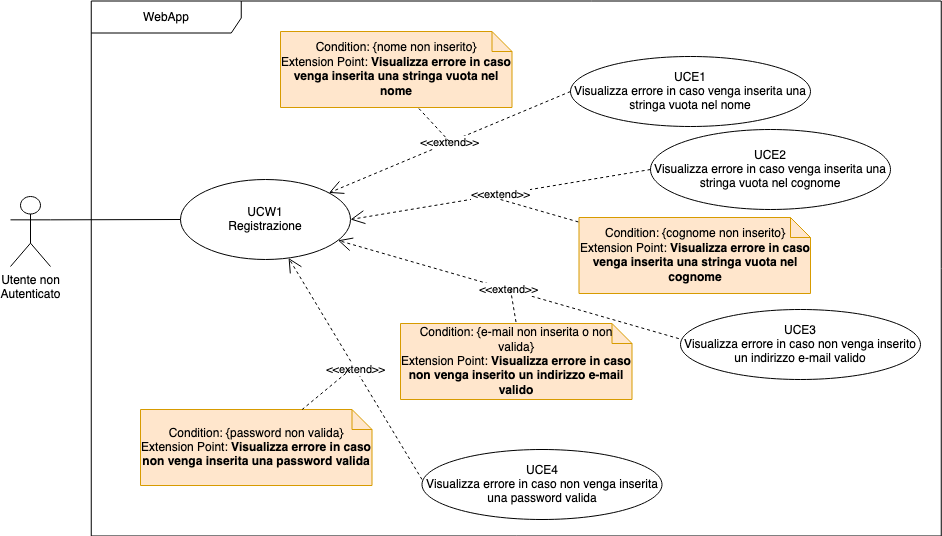
\includegraphics[scale=0.5]{UC_images/UCW1.png}
\caption{UCW1 – Registrazione}
\end{figure}
\begin{itemize}
\item \textbf{Descrizione}: L'utente non autenticato si registra nella piattaforma Sweeat.
\item \textbf{Attore primario}: Utente non autenticato.
\item \textbf{Precondizione}: L'utente non è ancora autenticato presso il sistema.
\item \textbf{Postcondizione}: L’utente possiede un account con cui può accedere al sistema, contraddistinto da una username ed una password.

\item \textbf{Scenario principale}:
\begin{enumerate}
\item L’utente accede al sistema;
\item L’utente seleziona la funzionalità “Registrati”;
\item L'utente inserisce i campi dati obbligatori: Nome e Cognome;
\item L’utente inserisce un indirizzo e-mail univoco nel campo username non ancora utilizzato con cui accedere al sistema; 
\item L’utente inserisce una password per accedere al sistema;
\item Affinché la registrazione vada a buon fine, l’utente dovrà cliccare su “Registrati”.
\end{enumerate}

\item \textbf{Estensioni}:
\begin{itemize}
\item{Nel caso in cui l'utente non inserisca correttamente il suo nome}
\begin{enumerate}
	\item L'utente non viene registrato nel sistema;
	\item Viene mostrato un messaggio d'errore che indica che il nome non è stato inserito correttamente (UCE1 §).
\end{enumerate}
\item{Nel caso in cui l'utente non inserisca correttamente il suo cognome}
\begin{enumerate}
	\item L'utente non viene registrato nel sistema;
	\item Viene mostrato un messaggio d'errore che indica che il cognome non è stato inserito correttamente (UCE2 §).
\end{enumerate}
\item Nel caso in cui l’utente inserisca un indirizzo e-mail non esistente, già presente a sistema o lasci il campo vuoto
\begin{enumerate}
	\item L’utente non viene registrato nel sistema;
	\item Viene mostrato un messaggio d’errore che indica che l'indirizzo e-mail inserito non è corretto (UCE3 §).
\end{enumerate}
\item Nel caso in cui l’utente provi a registrarsi inserendo una password più breve di 8 caratteri
\begin{enumerate}
	\item L’utente non viene registrato nel sistema;
	\item Viene mostrato un messaggio d’errore che indica che non è stata inserita alcuna password (UCE4 §).
\end{enumerate}
\end{itemize}
\end{itemize}
	
	\subsubsection{UCW2 - Login}
	\subsubsection{UCW2 - Login}
\begin{figure}[!h]
\centering
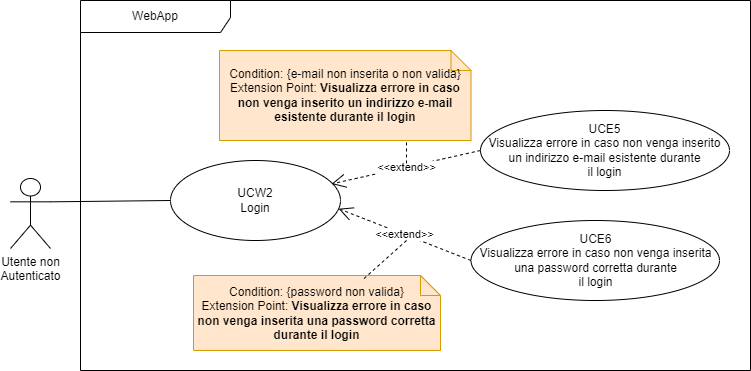
\includegraphics[scale=0.5]{UC_images/UCW2.png}
\caption{UCW2 - Login}
\end{figure}
\begin{itemize}
\item \textbf{Descrizione}: L'utente non autenticato accede alla piattaforma Sweeat.
\item \textbf{Attore primario}: Utente non autenticato.
\item \textbf{Precondizione}: L'utente non è ancora autenticato presso il sistema.
\item \textbf{Postcondizione}: L’utente ha effettuato l’accesso al sistema ed è all’interno del suo account.

\item \textbf{Scenario principale}:
\begin{enumerate}
\item L’utente accede al sistema;
\item L’utente seleziona la voce “Login”;
\item L’utente inserisce l’indirizzo e-mail con cui è registrato al sistema;
\item L’utente inserisce la password d’accesso; 
\item L’utente seleziona la voce “Accedi”. 
\end{enumerate}

\item \textbf{Estensioni}:
\begin{itemize}
\item Viene inserito un indirizzo e-mail errato 
\begin{enumerate}
	\item L’utente non può accedere al sistema;
	\item Viene mostrato un messaggio d’errore che indica che l'indirizzo e-mail inserito con cui accedere al sistema non è corretto (UCE5 §3.19). 
\end{enumerate}
\item Viene inserita una password errata
\begin{enumerate}
	\item L’utente non può accedere al sistema;
	\item Viene mostrato un messaggio d’errore che indica che la password inserita non è corretta (UCE6 §3.20).
\end{enumerate}
\end{itemize}
\end{itemize}
	
	\subsubsection{UCW3 - Recupero Password}
	\subsubsection{UCW3 – Recupero Password}
\begin{figure}[!h]
\centering
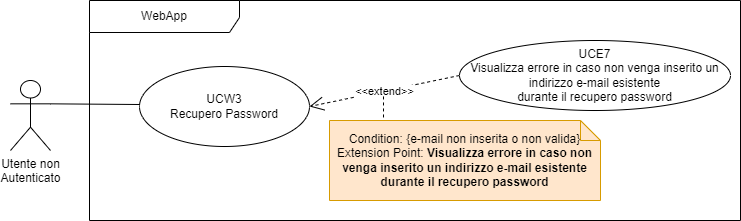
\includegraphics[scale=0.5]{UC_images/UCW3.png}
\caption{UCW3 - Recupero Password}
\end{figure}
\begin{itemize}
\item \textbf{Descrizione}: L'utente non autenticato vuole recuperare la password di accesso alla piattaforma Sweeat.
\item \textbf{Attore primario}: Utente non autenticato.
\item \textbf{Precondizione}: L’utente non è ancora autenticato presso il sistema.
\item \textbf{Postcondizione}: L’utente ha la possibilità di recuperare la password tramite l'indirizzo e-mail con cui è registrato nella piattaforma.

\item \textbf{Scenario principale}:
\begin{enumerate}
\item L’utente accede al sistema;
\item L’utente seleziona la voce “Login”;
\item L’utente clicca sulla voce “Password dimenticata”;
\item L’utente inserisce l’indirizzo e-mail da cui recuperare la password;
\item L’utente clicca su “Recupera password”. 
\end{enumerate}

\item \textbf{Estensioni}:
\begin{itemize}
\item Viene inserito un indirizzo e-mail non valido 
\begin{enumerate}
	\item L’utente non può recuperare la password;
	\item Viene mostrato un messaggio d’errore che indica che l’indirizzo e-mail inserito non è corretto (UCE7 §3.21).
\end{enumerate}
\end{itemize}
\end{itemize}

\pagebreak
	
	\subsection{UCW4 - Area Personale}
	\subsection{UCW4 - Gestione Dati Personali}
\begin{figure}[!h]
\centering
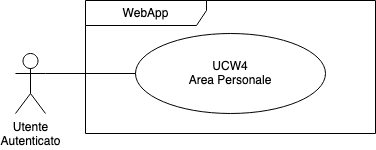
\includegraphics[scale=0.5]{UC_images/UCW4.png}
\caption{UCW4 - Gestione Dati Personali}
\end{figure}
\begin{itemize}
\item \textbf{Descrizione}: L'utente è autenticato nella piattaforma Sweeat e può gestire i suoi dati personali.
\item \textbf{Attore primario}: Utente Autenticato.
\item \textbf{Precondizione}: L'utente è autenticato nella piattaforma.
\item \textbf{Postcondizione}: L'utente accede all'area per gestire i suoi dati personali inseriti in fase di registrazione.

\item \textbf{Scenario principale}:
\begin{enumerate}
\item L'utente autenticato clicca l'icona per accedere alla sua Area Personale;
\item Una volta entrato nell'Area Personale, può gestire i suoi dati.
\end{enumerate}

\item \textbf{Sottocasi}:
\begin{enumerate}
	\item Collegare l'account personale di Instagram (UCW4.1 \S 3.5.1).
	\item Collegare l'account personale di TikTok (UCW4.2 \S 3.5.2).
	\item Modificare la password (UCW4.3 \S 3.5.3). 
\end{enumerate}
\end{itemize}
\begin{figure}[!h]
\centering
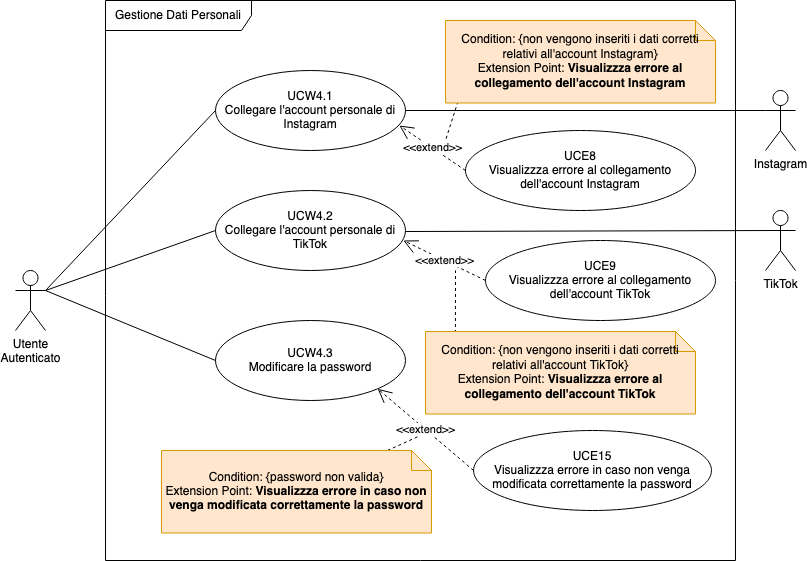
\includegraphics[scale=0.5]{UC_images/UCW4-1.png}
\caption{Sottocasi UCW4}
\end{figure}
\subsubsection{UCW4.1 - Collegare l'Account Instagram}
\begin{itemize}
\item \textbf{Descrizione}: L'utente autenticato collega il proprio account Instagram al profilo.
\item \textbf{Attore primario}: Utente autenticato.
\item \textbf{Attore secondario}: Instagram.
\item \textbf{Precondizione}: L’utente è autenticato nel sistema.
\item \textbf{Postcondizione}: L’utente ha collegato il suo account Instagram al sistema.

\item \textbf{Scenario principale}:
\begin{enumerate}
\item L’utente collega il suo account personale di Instagram;
\item Per confermare l’azione, l’utente deve cliccare su “Salva”. 
\end{enumerate}

\item \textbf{Estensioni}:
\begin{itemize}
\item Il collegamento all’account Instagram non va a buon fine
\begin{enumerate}
	\item L’utente prova a collegare il proprio account Instagram all’account registrato nel sistema, cliccando il bottone “Instagram”;
	\item L’accesso alla piattaforma Instagram non va a buon fine, poiché non vengono inseriti i dati di accesso corretti (UCE8 §3.22).
	%\item All’utente viene offerta la possibilità di effettuare un nuovo collegamento
\end{enumerate}
\end{itemize}
\end{itemize}

\subsubsection{UCW4.2 - Collegare l'Account TikTok}
\begin{itemize}
\item \textbf{Descrizione}: L'utente autenticato collega il proprio account TikTok al profilo.
\item \textbf{Attore primario}: Utente autenticato.
\item \textbf{Attore secondario}: TikTok.
\item \textbf{Precondizione}: L’utente è autenticato nel sistema.
\item \textbf{Postcondizione}: L’utente ha collegato il suo account TikTok al sistema.

\item \textbf{Scenario principale}:
\begin{enumerate}
\item L’utente collega il suo account personale di TikTok;
\item Per confermare l’azione, l’utente deve cliccare su “Salva”. 
\end{enumerate}

\item \textbf{Estensioni}:
\begin{itemize}
\item Il collegamento all’account TikTok non va a buon fine
\begin{enumerate}
	\item L’utente prova a collegare il proprio account TikTok all’account registrato nel sistema, cliccando il bottone TikTok;
	\item L’accesso alla piattaforma TikTok non va a buon fine, poiché non vengono inseriti i dati di accesso corretti (UCE9 §3.23).
\end{enumerate}
\end{itemize}
\end{itemize}

\subsubsection{UCW4.3 - Modifica della password}
\begin{itemize}
\item \textbf{Descrizione}: L'utente autenticato modifica la password con cui accedere al sistema.
\item \textbf{Attore primario}: Utente autenticato.
\item \textbf{Precondizione}: L’utente è autenticato nel sistema.
\item \textbf{Postcondizione}: L’utente ha modificato con successo la password per l’accesso al sistema.

\item \textbf{Scenario principale}:
\begin{enumerate}
\item L’utente digita la nuova password nel campo password;
\item L’utente clicca su “Salva” per aggiornare la password con cui accedere al sistema.
\end{enumerate}

\item \textbf{Estensioni}:
\begin{itemize}
\item Viene inserita una password con meno di 8 caratteri
\begin{enumerate}
	\item L'utente inserisce una password non valida (UCE15 §3.29).
\end{enumerate}
\end{itemize}
\end{itemize}

\pagebreak
	
	\subsection{UCW5 - Proposta profilo Instagram}
	%\subsection{UCW5 - Proposta profilo Instagram}
\begin{figure}[!h]
\centering
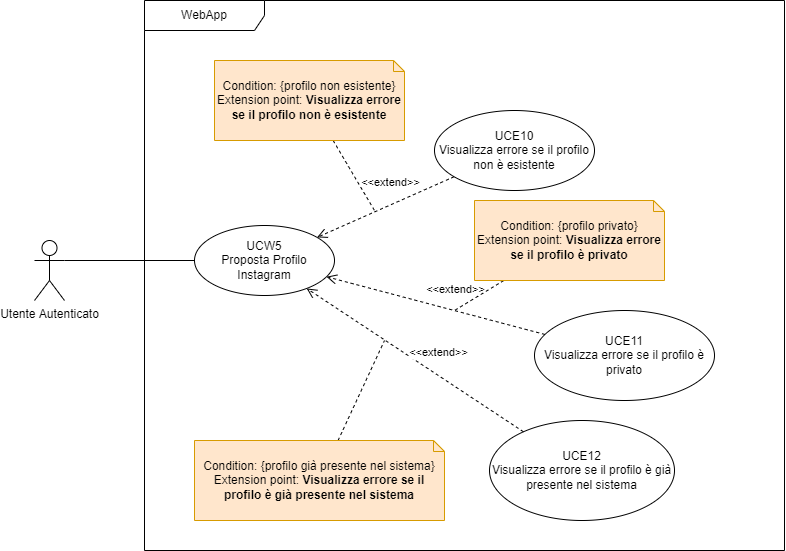
\includegraphics[scale=0.5]{UC_images/UCW5.png}
\caption{UCW5 - Proposta profilo Instagram}
\end{figure}
\begin{itemize}
	\item \textbf{Descrizione}: L'utente autenticato propone uno specifico profilo Instagram da cui effettuare il crawling dei dati.
    \item \textbf{Attore primario}: Utente autenticato.
    \item \textbf{Precondizione}: Il sistema possiede una lista di profili instagram da cui effettuare il crawling dei dati.
    \item \textbf{Postcondizione}: Alla lista di profili da cui effettuare il crawling viene aggiunto il profilo indicato dall’utente e tutti i profili pubblici seguiti dal profilo suggerito.
    \item \textbf{Scenario principale}: 
    \begin{enumerate}
        \item L'utente autenticato accede al sistema;
        \item L’utente seleziona la funzionalità suggerisci un profilo instagram;
        \item L’utente inserisce uno username valido di un profilo instagram pubblico.
    \end{enumerate}
    \item \textbf{Estensioni}:
    \begin{itemize}
        \item Nel caso in cui l’utente inserisca uno username non esistente:
        \begin{enumerate}
            \item Lo username non viene inserito nella lista;
            \item Viene visualizzato un messaggio di errore nella proposta di profilo (UCE10 §3.24);
            \item Viene fornita all’utente la possibilità di modificare lo username inserito.
        \end{enumerate}
        \item Nel caso in cui l’utente inserisca lo username di un profilo privato:
        \begin{enumerate}
            \item Lo username non viene inserito nella lista;
            \item Viene visualizzato un messaggio di errore nella proposta di profilo (UCE11 §3.25).
        \end{enumerate}
        \item Nel caso in cui venga inserito lo username di un profilo pubblico già presente nel sistema:
        \begin{enumerate}
            \item Lo username non viene inserito nella lista.
            \item Viene visualizzato un messaggio di errore nella proposta di profilo (UCE12 §3.26).
        \end{enumerate} 
    \end{itemize}
\end{itemize}

% \subsection{UC3.1 - Verifica privacy profilo}
% \begin{itemize}
%     \item \textbf{Attore primario}: Utente autenticato.
%     \item \textbf{Attore secondario}: Social generico.
%     \item \textbf{Precondizione}: L’utente ha richiesto l’aggiunta di un profilo social fornendone il link.
%     \item \textbf{Postcondizione}: Il sistema sa se il profilo suggerito è pubblico o privato.

%     \item \textbf{Scenario principale}: 
%     \begin{enumerate}
%         \item Il sistema chiede al social in questione se il profilo proposto è pubblico o privato;
%         \item Il social in questione invia una risposta dicendo se il profilo è pubblico o privato.
%     \end{enumerate}

%     \item \textbf{Inclusioni}:
%     \begin{enumerate}
%         \item Verifica validità link (UC3.2 §).
%     \end{enumerate}
% \end{itemize}

% \subsection{UC3.2 - Verifica validità link}
% \begin{itemize}
%     \item \textbf{Attore primario}: Utente autenticato.
%     \item \textbf{Attore secondario}: Social generico.
%     \item \textbf{Precondizione}: L’utente ha richiesto l’aggiunta di un profilo social fornendone il link.
%     \item \textbf{Postcondizione}: Il sistema sa se il link fornito è valido.

%     \item \textbf{Scenario principale}: 
%     \begin{enumerate}
%         \item Il sistema chiede al social in questione se il link è valido;
%         \item Il social in questione invia una risposta dicendo se il link è valido o meno.
%     \end{enumerate}
% \end{itemize}
	
	\subsection{UCW6 - Proposta profilo TikTok}
	\subsection{UCW6 - Proposta profilo TikTok}
\begin{figure}[!h]
\centering
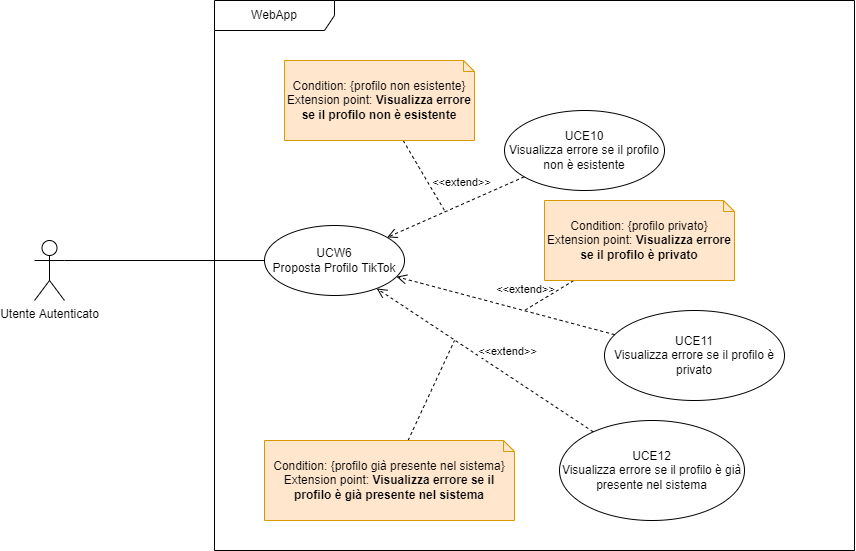
\includegraphics[scale=0.5]{UC_images/UCW6.png}
\caption{UCW6 - Proposta profilo TikTok}
\end{figure}
\begin{itemize}
	\item \textbf{Descrizione}: L'utente autenticato propone uno specifico profilo TikTok da cui effettuare il crawling dei dati.
    \item \textbf{Attore primario}: Utente autenticato.
    \item \textbf{Precondizione}: Il sistema possiede una lista di profili TikTok da cui effettuare il crawling dei dati.
    \item \textbf{Postcondizione}: Alla lista di profili da cui effettuare il crawling viene aggiunto il profilo indicato dall’utente e tutti i profili pubblici seguiti dal profilo suggerito.
    \item \textbf{Scenario principale}: 
    \begin{enumerate}
        \item L'utente autenticato accede al sistema;
        \item L’utente seleziona la funzionalità suggerisci un profilo TikTok;
        \item L’utente inserisce uno username valido di un profilo TikTok pubblico.
    \end{enumerate}
    \item \textbf{Estensioni}:
    \begin{itemize}
        \item Nel caso in cui l’utente inserisce uno username non esistente:
        \begin{enumerate}
            \item Lo username non viene inserito nella lista;
            \item Viene visualizzato un messaggio di errore nella proposta di profilo (UCE10 §);
            \item Viene fornita all’utente la possibilità di modificare lo username inserito.
        \end{enumerate}
        \item Nel caso in cui l’utente inserisce lo username di un profilo privato:
        \begin{enumerate}
            \item Lo username non viene inserito nella lista;
            \item Viene visualizzato un messaggio di errore nella proposta di profilo (UCE11 §).
        \end{enumerate}
        \item Nel caso in cui viene inserito lo username di un profilo pubblico già presente nel sistema:
        \begin{enumerate}
            \item Lo username non viene inserito nella lista.
            \item Viene visualizzato un messaggio di errore nella proposta di profilo (UCE12 §).
        \end{enumerate} 
    \end{itemize}
\end{itemize}

\pagebreak
	
	\subsection{UCW7 - Visualizza Classifica}
	\subsection{UCW7 - Visualizza Classifica}
\begin{figure}[!h]
\centering
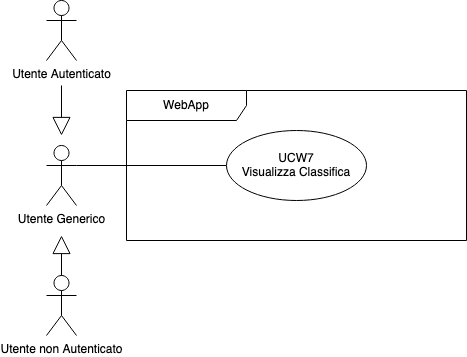
\includegraphics[scale=0.5]{UC_images/UCW7.png}
\caption{UCW7 - Visualizza Classifica}
\end{figure}
\begin{center}
\end{center}
\begin{itemize}
	\item \textbf{Descrizione}: L'utente generico visualizza la classifica dei locali presenti sulla piattaforma Sweeat.
    \item \textbf{Attore primario}: Utente generico.
    \item \textbf{Precondizione}: L’utente si trova all’interno della piattaforma Sweeat.
    \item \textbf{Postcondizione}: L’utente visualizza a schermo la classifica dei migliori locali gastronomici prodotta dal sistema senza alcun filtro applicato e con i parametri di ordinamento di default.
    \item \textbf{Scenario principale}: 
    \begin{enumerate}
        \item Un utente generico accede al sistema;
        \item L’utente seleziona la funzionalità visualizza classifica.
    \end{enumerate}
    \item \textbf{Sottocasi}:
    \begin{enumerate}
        \item Visualizza nomi locali (UCW7.1 §3.9.1);
        \item Visualizza punteggi totali (UCW7.2 §3.9.2);
        \item Visualizza categorie (UCW7.3 §3.9.3);
        \item Visualizza foto (UCW7.4 §3.9.5).
    \end{enumerate}
\end{itemize}


	
	\subsection{UCW8 - Filtra classifica}
	%\subsection{UCW8 - Filtra classifica}
\begin{figure}[!h]
\centering
    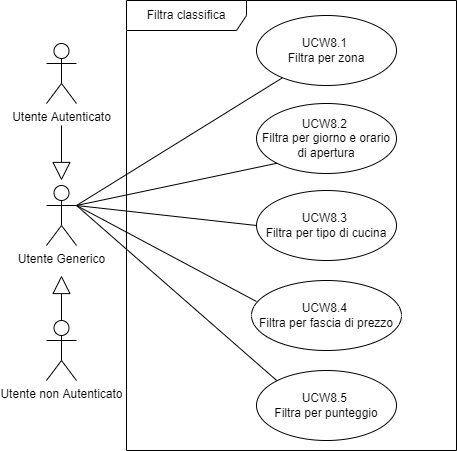
\includegraphics[scale=0.5]{UC_images/UCW8.png}
    \caption{UCW8 - Filtra classifica}
\end{figure}
\begin{itemize}
	\item \textbf{Descrizione}: L'utente generico filtra la classifica con i risultati dei locali.
    \item \textbf{Attore primario}: Utente generico.
    \item \textbf{Precondizione}: L’utente sta visualizzando la classifica (UCW7 §3.8).
    \item \textbf{Postcondizione}: L’utente visualizza a schermo la classifica dei migliori locali gastronomici che rientrano all’interno dei filtri inseriti.
    \item \textbf{Scenario principale}: 
    \begin{enumerate}
        \item L’utente clicca il pulsante “Filtra Classifica”;
        \item L’utente applica dei filtri;
        \item L’utente clicca il pulsante “Applica Filtri”.
    \end{enumerate}

    \item \textbf{Sottocasi}:
    \begin{enumerate}
        \item Filtra per zona (UCW8.1 §3.9.1);
        \item Filtra per giorno e orario di apertura (UCW8.2 §3.9.2);
        \item Filtra per tipo di cucina (UCW8.3 §3.9.3);
        \item Filtra per fascia di prezzo (UCW8.4 §3.9.4);
        \item Filtra per punteggio (UCW8.5 §3.9.5).
    \end{enumerate}

    \item \textbf{Estensioni}:
    \begin{itemize}
        \item Nel caso in cui non ci sia nemmeno un locale che rispetta i filtri applicati:
        \begin{enumerate}
            \item Viene visualizzato un messaggio che informa l’utente del fatto che nessun locale rientra nei filtri inseriti (UCE13 §3.27);
            \item Viene fornita la possibilità di modificare i filtri.
        \end{enumerate}
    \end{itemize}
\end{itemize}

\begin{figure}[!h]
\centering
    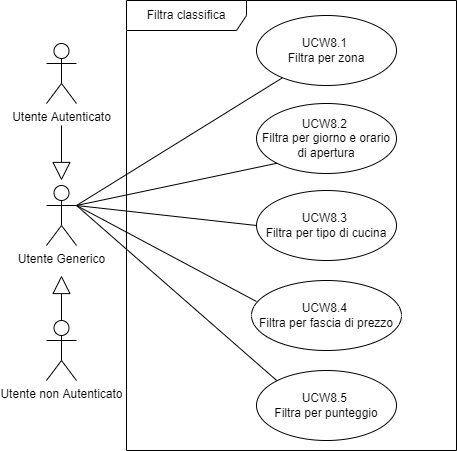
\includegraphics[scale=0.5]{UC_images/UCW8-.png}
    \caption{Sottocasi UCW8}
\end{figure}

\subsubsection{UCW8.1 - Filtra per zona}
\begin{itemize}
	\item \textbf{Descrizione}: L'utente generico filtra la classifica per zona.
    \item \textbf{Attore primario}: Utente generico.
    \item \textbf{Precondizione}: L’utente sta visualizzando la classifica (UCW7 §3.8) e ha premuto il pulsante “Filtra Classifica”.
    \item \textbf{Postcondizione}: Il filtro in questione viene applicato.
    \item \textbf{Scenario principale}: 
    \begin{enumerate}
        \item L’utente digita il nome di uno o più luoghi;
        \item L’utente preme il pulsante invio.
    \end{enumerate}
\end{itemize}

\subsubsection{UCW8.2 - Filtra per giorno e orario di apertura}
\begin{itemize}
	\item \textbf{Descrizione}: L'utente generico filtra la classifica per giorno e orario di apertura.
    \item \textbf{Attore primario}: Utente generico.
    \item \textbf{Precondizione}: L’utente sta visualizzando la classifica (UCW7 §3.8) e ha premuto il pulsante “Filtra Classifica”.
    \item \textbf{Postcondizione}: Il filtro in questione viene applicato.
    \item \textbf{Scenario principale}: 
    \begin{enumerate}
        \item L’utente seleziona uno o più giorni della settimana da un checkbox;
        \item L’utente inserisce uno o più orari;
        \item L’utente clicca il pulsante “OK”.
    \end{enumerate}
\end{itemize}

\subsubsection{UCW8.3 - Filtra per tipo di cucina}
\begin{itemize}
	\item \textbf{Descrizione}: L'utente generico filtra la classifica per tipo di cucina.
    \item \textbf{Attore primario}: Utente generico.
    \item \textbf{Precondizione}: L’utente sta visualizzando la classifica (UCW7 §3.8) e ha premuto il pulsante “Filtra Classifica”.
    \item \textbf{Postcondizione}: Il filtro in questione viene applicato.
    \item \textbf{Scenario principale}: 
    \begin{enumerate}
        \item L’utente seleziona uno o più tipi di cucina tra quelli proposti tramite un checkbox;
        \item L’utente clicca il pulsante “OK”.
    \end{enumerate}
\end{itemize}

\subsubsection{UCW8.4 - Filtra per fascia di prezzo}
\begin{itemize}
	\item \textbf{Descrizione}: L'utente generico filtra la classifica per fascia di prezzo.
    \item \textbf{Attore primario}: Utente generico.
    \item \textbf{Precondizione}: L’utente sta visualizzando la classifica (UCW7 §3.8) e ha premuto il pulsante “Filtra Classifica”.
    \item \textbf{Postcondizione}: Il filtro in questione viene applicato.
    \item \textbf{Scenario principale}: 
    \begin{enumerate}
        \item L’utente inserisce il valore minimo della fascia di prezzo;
        \item L’utente inserisce il valore massimo della fascia di prezzo;
        \item L’utente clicca il pulsante “OK”.
    \end{enumerate}
\end{itemize}

\subsubsection{UCW8.5 - Filtra per punteggio}
\begin{itemize}
	\item \textbf{Descrizione}: L'utente generico filtra la classifica per punteggio.
    \item \textbf{Attore primario}: Utente generico.
    \item \textbf{Precondizione}: L’utente sta visualizzando la classifica (UCW7 §3.8) e ha premuto il pulsante “Filtra Classifica”.
    \item \textbf{Postcondizione}: Il filtro in questione viene applicato.
    \item \textbf{Scenario principale}: 
    \begin{enumerate}
        \item L’utente inserisce il punteggio minimo;
        \item L’utente inserisce il punteggio massimo;
        \item L’utente clicca il pulsante “OK”.
    \end{enumerate}
\end{itemize}

%\clearpage 
	
	\subsection{UCW9 - Modifica parametri di ordinamento classifica}
	\subsection{UCW9 - Modifica parametri di ordinamento classifica}
\begin{figure}[!h]
\centering
    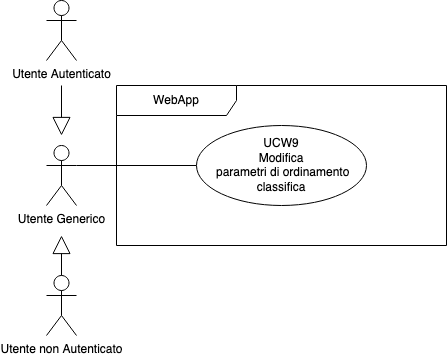
\includegraphics[scale=0.5]{UC_images/UCW9.png}
    \caption{UCW9 - Modifica parametri di ordinamento classifica}
\end{figure}
\begin{itemize}
	\item \textbf{Descrizione}: L'utente generico modifica i parametri di ordinamento della classifica con i risultati dei locali.
    \item \textbf{Attore primario}: Utente generico.
    \item \textbf{Precondizione}: L’utente sta visualizzando la classifica (UCW7 §3.8).
    \item \textbf{Postcondizione}: L’utente visualizza a schermo la classifica dei migliori locali gastronomici riordinata in base ai parametri di ordinamento inseriti.
    \item \textbf{Scenario principale}: 
    \begin{enumerate}
        \item L’utente clicca il pulsante “modifica parametri di ordinamento”;
        \item L’utente modifica i parametri di ordinamento;
        \item L’utente cicca il pulsante “applica parametri”.
    \end{enumerate}

    \item \textbf{Sottocasi}:
    \begin{enumerate}
        \item Modifica peso dei social (UCW9.1 §3.10.1);
        \item Modifica peso dei tipi di contenuto (UCW9.2 §3.10.2).
    \end{enumerate}

\end{itemize}

\begin{figure}[!h]
\centering
    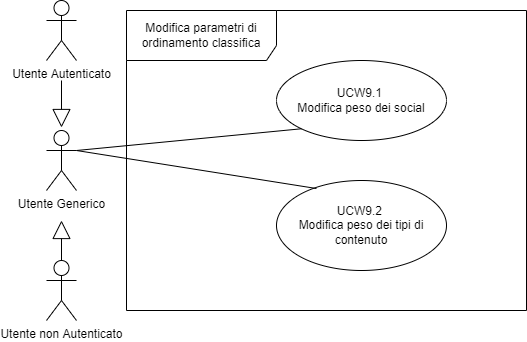
\includegraphics[scale=0.5]{UC_images/UCW9-.png}
    \caption{Sottocasi UCW9}
\end{figure}

\subsubsection{UCW9.1 - Modifica peso dei social }
\begin{itemize}
	\item \textbf{Descrizione}: L'utente generico modifica l'ordinamento della classifica in base al peso dei social.
    \item \textbf{Attore primario}: Utente generico.
    \item \textbf{Precondizione}: L’utente sta visualizzando la classifica (UCW7 §3.8) e ha premuto il pulsante “Modifica Parametri di Ordinamento”.
    \item \textbf{Postcondizione}: Il parametro in questione viene applicato.
    \item \textbf{Scenario principale}: 
    \begin{enumerate}
        \item L’utente modifica il peso in percentuale che forniscono i contenuti di ciascun social tramite una barra percentuale;
        \item L’utente clicca il pulsante “OK”.
    \end{enumerate}
\end{itemize}

\subsubsection{UCW9.2 - Modifica peso dei tipi di contenuto}
\begin{itemize}
	\item \textbf{Descrizione}: L'utente generico modifica l'ordinamento della classifica in base al peso dei tipi di contenuto.
    \item \textbf{Attore primario}: Utente generico.
    \item \textbf{Precondizione}: L’utente sta visualizzando la classifica (UCW7 §3.8) e ha premuto il pulsante “modifica parametri di ordinamento”.
    \item \textbf{Postcondizione}: Il parametro in questione viene applicato.
    \item \textbf{Scenario principale}: 
    \begin{enumerate}
        \item L’utente modifica il peso in percentuale che forniscono i tipi di contenuto (foto, post, stories, commenti) tramite una barra percentuale;
        \item L’utente clicca il pulsante “OK”.
    \end{enumerate}
\end{itemize}

\pagebreak
	
	\subsection{UCW10 - Ricerca di un locale tramite nome}
	%\subsection{UCW10 - Ricerca di un locale tramite nome}
\begin{figure}[!h]
\centering
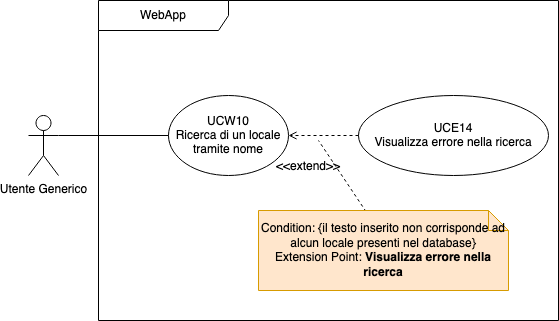
\includegraphics[scale=0.5]{UC_images/UCW10.png} 
\caption{UCW10 - Ricerca di un locale tramite nome}
\end{figure}
\begin{itemize}
    \item \textbf{Descrizione}: L'utente generico effettua la ricerca di un locale tramite il suo nome.
    \item \textbf{Attore primario}: Utente generico.
    \item \textbf{Precondizione}: L'utente si trova all’interno della piattaforma Sweeat.
    \item \textbf{Postcondizione}: Viene visualizzato la lista dei locali ricercati.
    \item \textbf{Scenario principale}: 
    \begin{enumerate}
        \item L’utente va nella barra di ricerca della piattaforma;
        \item L’utente digita il nome del locale da cercare;
        \item L’utente clicca sul bottone di ricerca.
    \end{enumerate}
    \item \textbf{Estensioni}:
    \begin{itemize}
        \item Nel caso in cui l’utente inserisca un testo non corrispondente a nessun locale presente nel database
	\begin{enumerate}  
		\item L’utente va nella barra di ricerca della piattaforma;
        \item L’utente digita il nome del locale da cercare;
        \item L’utente clicca sul bottone di ricerca; 
        \item Viene mostrato un messaggio d'errore, nel caso non sia presente alcun locale simile al locale ricercato(UCE14 §3.28).
    	%Visualizzazione di un messaggio informando che non è presente nessun locale con tale nome e viene suggerita una lista di locali simili a quello ricercato.   
    \end{enumerate}
    \end{itemize}    
\end{itemize}

\subsection{UCW11 - Visualizza informazioni locale}
\begin{figure}[!h]
\centering
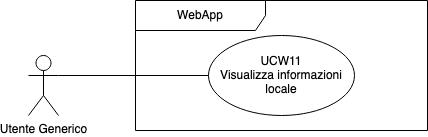
\includegraphics[scale=0.5]{UC_images/UCW11.png} 
\caption{UCW11 - Visualizza informazioni locale}
\end{figure}
\begin{itemize}
    \item \textbf{Descrizione}: L'utente generico visualizza le informazioni di un locale.
    \item \textbf{Attore primario}: Utente generico.
    \item \textbf{Precondizione}: L'utente ha svolto la funzione di ricerca di un locale o sta visualizzando la classifica dei locali.
    \item \textbf{Postcondizione}: Vengono visualizzate le informazioni di un locale:
    \begin{enumerate}
        \item Nome del locale;
        \item Descrizione del locale;
        \item Indirizzo del locale;
        \item Punteggio del locale;
        \item Numero di telefono del locale;
        \item Sito web del locale.
        \end{enumerate}
    \item \textbf{Scenario principale}: 
    \begin{enumerate}
    \item L'utente seleziona un locale tra quelli presenti nella lista;
    \item Il sistema mostrerà all'utente le informazioni relative al locale scelto.
    \end{enumerate}
\end{itemize}

	
	\subsection{UCW11 - Visualizza informazioni locale}
	%\subsection{UCW11 - Visualizza informazioni locale}
\begin{figure}[!h]
\centering
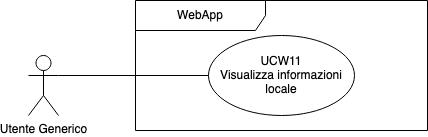
\includegraphics[scale=0.5]{UC_images/UCW11.png} 
\caption{UCW11 - Visualizza informazioni locale}
\end{figure}
\begin{itemize}
    \item \textbf{Descrizione}: L'utente generico visualizza le informazioni di un locale.
    \item \textbf{Attore primario}: Utente generico.
    \item \textbf{Precondizione}: L'utente ha svolto la funzione di ricerca di un locale o sta visualizzando la classifica dei locali.
    \item \textbf{Postcondizione}: Vengono visualizzate le informazioni di base di un locale:
    \begin{enumerate}
        \item Visualizza informazioni generali;
        \item Visualizza punteggio locale;
        \item Visualizza dati estratti;
        \item Visualizza icona preferiti.
    \end{enumerate}   
	\item \textbf{Sottocasi}:    
	\begin{enumerate}  
		\item Visualizza informazioni generali (UCW11.1 \S{}3.12.1);
		\item Visualizza punteggio locale (UCW11.2 \S{}3.12.2);
		\item Visualizza contenuti estratti (UCW11.3 \S{}3.12.3);
		\item Visualizza icona preferiti (UCW11.4 \S{}3.12.4).
	\end{enumerate}
    \item \textbf{Scenario principale}: 
    \begin{enumerate}
	\item L'utente visualizza la classifica dei locali presenti nel sistema;
    \item Per ciascun locale, la lista mostrerà alcune informazioni di base.
    \end{enumerate}
\end{itemize}

\begin{figure}[!h]
	\centering
		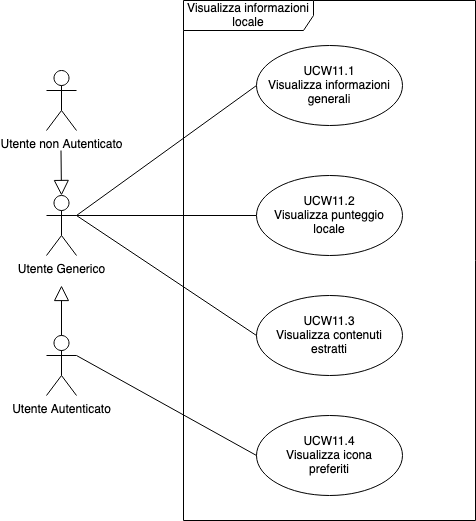
\includegraphics[scale=0.5]{UC_images/UCW11-.png} 
		\caption{Sottocasi UCW11}
\end{figure}  

\subsubsection{UCW11.1 - Visualizza informazioni generali}
\begin{itemize}
    \item \textbf{Descrizione}: L'utente generico visualizza le informazioni di un locale.
    \item \textbf{Attore primario}: Utente generico.
    \item \textbf{Precondizione}: L'utente ha svolto la funzione di ricerca di un locale o sta visualizzando la classifica dei locali.
    \item \textbf{Postcondizione}: Vengono visualizzate le principali informazioni di base di ciascun locale.
	\item \textbf{Sottocasi}:
	\begin{enumerate}
		\item Visualizza nome locale (UCW11.1.1 \S{}3.12.5);
		\item Visualizza posizione locale (UCW11.1.2 \S{}3.12.6);
		\item Visualizza categoria locale (UCW11.1.3 \S{}3.12.7);
		\item Visualizza orari di apertura locale (UCW11.1.4 \S{}3.12.8);
		\item Visualizza numero di telefono locale (UCW11.1.5 \S{}3.12.9);
		\item Visualizza sito web locale (UCW11.1.6 \S{}3.12.10).
	\end{enumerate}
    \item \textbf{Scenario principale}: 
    \begin{enumerate}
	\item L'utente visualizza la classifica dei locali, inseriti sotto forma di lista, presenti nel sistema;
    \item L'utente identifica un locale tra quelli presenti nella lista;
    \item Il sistema mostrerà all'utente le principali informazioni relative al locale scelto.
    \end{enumerate}
\end{itemize}

\begin{figure}[!h]
	\centering
	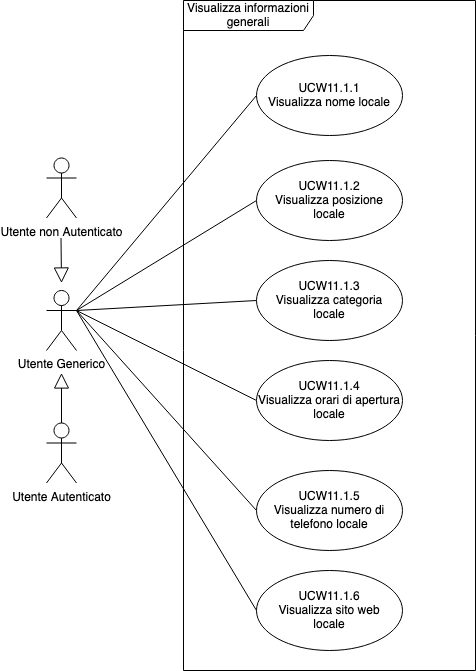
\includegraphics[scale=0.5]{UC_images/UCW11-1.png} 
	\caption{Sottocasi UCW11.1}
\end{figure}	

\subsubsection{UCW11.2 - Visualizza punteggio locale}
\begin{itemize}
    \item \textbf{Descrizione}: L'utente generico visualizza il punteggio di un locale.
    \item \textbf{Attore primario}: Utente generico.
    \item \textbf{Precondizione}: L'utente ha svolto la funzione di ricerca di un locale o sta visualizzando la classifica dei locali.
    \item \textbf{Postcondizione}: Viene visualizzato il punteggio del locale selezionato, calcolato analizzando i contenuti pubblicati sui social.
    \item \textbf{Sottocasi}:
	\begin{enumerate}
		\item Visualizza punteggio locale (UCW11.2.1 \S{}3.12.8);
		\item Visualizza punteggio contenuti multimediali (UCW11.2.2 \S{}3.12.12);
		\item Visualizza punteggio testi (UCW11.2.3 \S{}3.12.13);
		\item Visualizza punteggio emoticon (UCW11.2.4 \S{}3.12.14).
	\end{enumerate}
    \item \textbf{Scenario principale}: 
    \begin{enumerate}
	\item L'utente visualizza la classifica dei locali, inseriti sotto forma di lista, presenti nel sistema;    
    \item L'utente identifica un locale tra quelli presenti nella lista;
    \item Il sistema mostrerà all'utente la valutazione complessiva del locale scelto.
    \end{enumerate}
\end{itemize}

\begin{figure}[!h]
	\centering
	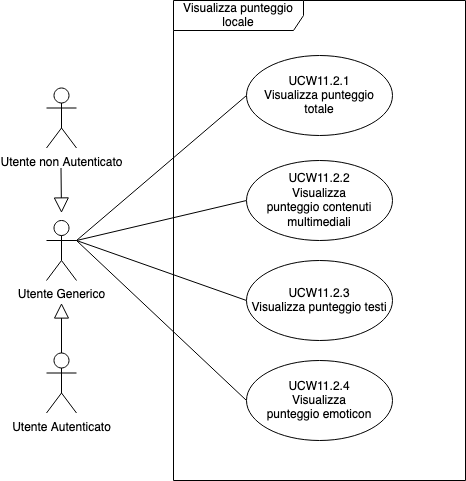
\includegraphics[scale=0.5]{UC_images/UCW11-2.png} 
	\caption{Sottocasi UCW11.2}
\end{figure}

\subsubsection{UCW11.3 - Visualizza dati estratti}
\begin{itemize}
    \item \textbf{Descrizione}: L'utente generico visualizza le informazioni di un locale.
    \item \textbf{Attore primario}: Utente generico.
    \item \textbf{Precondizione}: L'utente ha svolto la funzione di ricerca di un locale o sta visualizzando la classifica dei locali.
    \item \textbf{Postcondizione}: Vengono visualizzati i dati del locale selezionato estratti dai social.
    \item \textbf{Sottocasi}:
	\begin{enumerate}
		\item Visualizza foto (UCW11.3.1 \S{}3.12.15);
		\item Visualizza testi dei post (UCW11.3.2 \S{}3.12.16);
		\item Visualizza tag (UCW11.3.3 \S{}3.12.17).
	\end{enumerate}
    \item \textbf{Scenario principale}: 
    \begin{enumerate}
	\item L'utente autenticato visualizza la classifica dei locali, inseriti sotto forma di lista, presenti nel sistema;
    \item L'utente identifica un locale tra quelli presenti nella lista;
    \item Il sistema mostrerà all'utente i dati relativi al locale scelto, che sono stati estratti dai social.
    \end{enumerate}
\end{itemize}

\begin{figure}[!h]
	\centering
	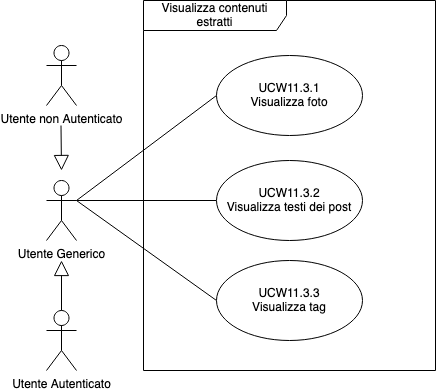
\includegraphics[scale=0.5]{UC_images/UCW11-3.png} 
	\caption{Sottocasi UCW11.3}
\end{figure}

\subsubsection{UCW11.4 - Visualizza icona preferiti}
\begin{itemize}
    \item \textbf{Descrizione}: L'utente autenticato visualizza l'icona “preferiti”.
    \item \textbf{Attore primario}: Utente autenticato.
    \item \textbf{Precondizione}: L'utente autenticato ha svolto la funzione di ricerca di un locale o sta visualizzando la classifica dei locali.
    \item \textbf{Postcondizione}: L'utente autenticato visualizza l'icona in questione per capire se ha inserito o meno il locale identificato nella lista dei preferiti e, nel caso il locale non sia presente nella lista, lo può aggiungere.
    \item \textbf{Scenario principale}: 
    \begin{enumerate}
    \item L'utente autenticato visualizza la classifica dei locali, inseriti sotto forma di lista, presenti nel sistema;
    \item L'utente autenticato identifica il locale di interesse tra quelli presenti nella lista;
    \item Il sistema mostrerà all'utente autenticato se quel locale è presente o meno nella sua lista dei preferiti e, nel caso non lo sia, lo può aggiungere (UCW12 \S{}3.13) o rimuovere (UCW13 \S{}3.14).
    \end{enumerate}
\end{itemize}

\subsubsection{UCW11.1.1 - Visualizza nome locale}
\begin{itemize}
    \item \textbf{Descrizione}: L'utente generico visualizza il nome di un locale.
    \item \textbf{Attore primario}: Utente generico.
    \item \textbf{Precondizione}: L'utente ha svolto la funzione di ricerca di un locale o sta visualizzando la classifica dei locali.
    \item \textbf{Postcondizione}: Viene visualizzato il nome del locale in questione.
    \item \textbf{Scenario principale}: 
    \begin{enumerate}
	\item L'utente visualizza la classifica dei locali, inseriti sotto forma di lista, presenti nel sistema;
    \item L'utente identifica un locale tra quelli presenti nella lista;
	\item Il sistema mostrerà all'utente il nome del locale identificato.
    \end{enumerate}
\end{itemize}

\subsubsection{UCW11.1.2 - Visualizza posizione locale}
\begin{itemize}
    \item \textbf{Descrizione}: L'utente generico visualizza la posizione di un locale.
    \item \textbf{Attore primario}: Utente generico.
    \item \textbf{Precondizione}: L'utente ha svolto la funzione di ricerca di un locale o sta visualizzando la classifica dei locali.
    \item \textbf{Postcondizione}: Viene visualizzata la posizione del locale in questione.
    \item \textbf{Scenario principale}: 
    \begin{enumerate}
	\item L'utente visualizza la classifica dei locali, inseriti sotto forma di lista, presenti nel sistema;
    \item L'utente identifica un locale tra quelli presenti nella lista;
	\item Il sistema mostrerà all'utente la posizione del locale identificato.
    \end{enumerate}
\end{itemize}

\subsubsection{UCW11.1.3 - Visualizza categoria locale}
\begin{itemize}
    \item \textbf{Descrizione}: L'utente generico visualizza la categoria di un locale.
    \item \textbf{Attore primario}: Utente generico.
    \item \textbf{Precondizione}: L'utente ha svolto la funzione di ricerca di un locale o sta visualizzando la classifica dei locali.
    \item \textbf{Postcondizione}: Viene visualizzata la categoria del locale in questione.
    \item \textbf{Scenario principale}: 
    \begin{enumerate}
	\item L'utente visualizza la classifica dei locali, inseriti sotto forma di lista, presenti nel sistema;
	\item L'utente identifica un locale tra quelli presenti nella lista;
	\item Il sistema mostrerà all'utente la categoria del locale identificato.
    \end{enumerate}
\end{itemize}

\subsubsection{UCW11.1.4 - Visualizza orari di apertura locale}
\begin{itemize}
    \item \textbf{Descrizione}: L'utente generico visualizza gli orari di apertura di un locale.
    \item \textbf{Attore primario}: Utente generico.
    \item \textbf{Precondizione}: L'utente ha svolto la funzione di ricerca di un locale o sta visualizzando la classifica dei locali.
    \item \textbf{Postcondizione}: Vengono visualizzati gli orari di apertura del locale selezionato.
    \item \textbf{Scenario principale}: 
    \begin{enumerate}
	\item L'utente visualizza la classifica dei locali, inseriti sotto forma di lista, presenti nel sistema;
	\item L'utente identifica un locale tra quelli presenti nella lista;
	\item Il sistema mostrerà all'utente gli orari di apertura del locale identificato.
    \end{enumerate}
\end{itemize}

\subsubsection{UCW11.1.5 - Visualizza numero di telefono locale}
\begin{itemize}
    \item \textbf{Descrizione}: L'utente generico visualizza il numero di telefono di un locale.
    \item \textbf{Attore primario}: Utente generico.
    \item \textbf{Precondizione}: L'utente ha svolto la funzione di ricerca di un locale o sta visualizzando la classifica dei locali.
    \item \textbf{Postcondizione}: Viene visualizzato il numero di telefono del locale selezionato.
    \item \textbf{Scenario principale}: 
    \begin{enumerate}
	\item L'utente visualizza la classifica dei locali, inseriti sotto forma di lista, presenti nel sistema;
	\item L'utente identifica un locale tra quelli presenti nella lista;
	\item Il sistema mostrerà all'utente il numero di telefono del locale identificato.
    \end{enumerate}
\end{itemize}

\subsubsection{UCW11.1.6 - Visualizza sito web locale}
\begin{itemize}
    \item \textbf{Descrizione}: L'utente generico visualizza il sito web di un locale.
    \item \textbf{Attore primario}: Utente generico.
    \item \textbf{Precondizione}: L'utente ha svolto la funzione di ricerca di un locale o sta visualizzando la classifica dei locali.
    \item \textbf{Postcondizione}: Viene visualizzato il sito web del locale in questione.
    \item \textbf{Scenario principale}: 
    \begin{enumerate}
	\item L'utente visualizza la classifica dei locali, inseriti sotto forma di lista, presenti nel sistema;
	\item L'utente identifica un locale tra quelli presenti nella lista;
	\item Il sistema mostrerà all'utente il sito web del locale identificato.
    \end{enumerate}
\end{itemize}

\subsubsection{UCW11.2.1 - Visualizza punteggio locale}
\begin{itemize}
    \item \textbf{Descrizione}: L'utente generico visualizza il punteggio totale di un locale.
    \item \textbf{Attore primario}: Utente generico.
    \item \textbf{Precondizione}: L'utente ha svolto la funzione di ricerca di un locale o sta visualizzando la classifica dei locali.
    \item \textbf{Postcondizione}: Viene visualizzato il punteggio totale del locale in questione.
    \item \textbf{Scenario principale}: 
    \begin{enumerate}
        \item L'utente visualizza la classifica dei locali, inseriti sotto forma di lista, presenti nel sistema;
        \item L'utente identifica un locale tra quelli presenti nella lista;
        \item Il sistema mostrerà all'utente il punteggio totale del locale identificato.
        \end{enumerate}
\end{itemize}
\subsubsection{UCW11.2.2 - Visualizza punteggio contenuti multimediali}
\begin{itemize}
    \item \textbf{Descrizione}: L'utente generico visualizza il punteggio dei contenuti multimediali di un locale.
    \item \textbf{Attore primario}: Utente generico.
    \item \textbf{Precondizione}: L'utente ha svolto la funzione di ricerca di un locale o sta visualizzando la classifica dei locali.
    \item \textbf{Postcondizione}: Viene visualizzato il punteggio dei contenuti multimediali del locale in questione.
    \item \textbf{Scenario principale}: 
    \begin{enumerate}
        \item L'utente visualizza la classifica dei locali, inseriti sotto forma di lista, presenti nel sistema;
        \item L'utente identifica un locale tra quelli presenti nella lista;
        \item Il sistema mostrerà all'utente il punteggio dei contenuti multimediali del locale identificato.
        \end{enumerate}
\end{itemize}
\subsubsection{UCW11.2.3 - Visualizza punteggio testi}
\begin{itemize}
    \item \textbf{Descrizione}: L'utente generico visualizza il punteggio dei testi di un locale.
    \item \textbf{Attore primario}: Utente generico.
    \item \textbf{Precondizione}: L'utente ha svolto la funzione di ricerca di un locale o sta visualizzando la classifica dei locali.
    \item \textbf{Postcondizione}: Viene visualizzato il punteggio dei testi del locale in questione.
    \item \textbf{Scenario principale}: 
    \begin{enumerate}
        \item L'utente visualizza la classifica dei locali, inseriti sotto forma di lista, presenti nel sistema;
        \item L'utente identifica un locale tra quelli presenti nella lista;
        \item Il sistema mostrerà all'utente il punteggio dei testi del locale identificato.
        \end{enumerate}
\end{itemize}

\subsubsection{UCW11.2.4 - Visualizza punteggio emoticon}
\begin{itemize}
    \item \textbf{Descrizione}: L'utente generico visualizza il punteggio delle emoticon di un locale.
    \item \textbf{Attore primario}: Utente generico.
    \item \textbf{Precondizione}: L'utente ha svolto la funzione di ricerca di un locale o sta visualizzando la classifica dei locali.
    \item \textbf{Postcondizione}: Viene visualizzato il punteggio delle emoticon del locale in questione.
    \item \textbf{Scenario principale}: 
    \begin{enumerate}
        \item L'utente visualizza la classifica dei locali, inseriti sotto forma di lista, presenti nel sistema;
        \item L'utente identifica un locale tra quelli presenti nella lista;
        \item Il sistema mostrerà all'utente il punteggio delle emoticon del locale identificato.
        \end{enumerate}
\end{itemize}

\subsubsection{UCW11.3.1 - Visualizza foto}
\begin{itemize}
    \item \textbf{Descrizione}: L'utente generico visualizza le foto di un locale.
    \item \textbf{Attore primario}: Utente generico.
    \item \textbf{Precondizione}: L'utente ha svolto la funzione di ricerca di un locale o sta visualizzando la classifica dei locali.
    \item \textbf{Postcondizione}: Viene visualizzato le foto del locale in questione.
    \item \textbf{Scenario principale}: 
    \begin{enumerate}
        \item L'utente visualizza la classifica dei locali, inseriti sotto forma di lista, presenti nel sistema;
        \item L'utente identifica un locale tra quelli presenti nella lista;
        \item Il sistema mostrerà all'utente le foto del locale identificato.
        \end{enumerate}
\end{itemize}
\subsubsection{UCW11.3.2 - Visualizza testi dei post}
\begin{itemize}
    \item \textbf{Descrizione}: L'utente generico visualizza i testi dei post di un locale.
    \item \textbf{Attore primario}: Utente generico.
    \item \textbf{Precondizione}: L'utente ha svolto la funzione di ricerca di un locale o sta visualizzando la classifica dei locali.
    \item \textbf{Postcondizione}: Viene visualizzato i testi dei post del locale in questione.
    \item \textbf{Scenario principale}: 
    \begin{enumerate}
        \item L'utente visualizza la classifica dei locali, inseriti sotto forma di lista, presenti nel sistema;
        \item L'utente identifica un locale tra quelli presenti nella lista;
        \item Il sistema mostrerà all'utente i testi dei post del locale identificato.
        \end{enumerate}
\end{itemize}
\subsubsection{UCW11.3.3 - Visualizza tag}
\begin{itemize}
    \item \textbf{Descrizione}: L'utente generico visualizza le tag di un locale.
    \item \textbf{Attore primario}: Utente generico.
    \item \textbf{Precondizione}: L'utente ha svolto la funzione di ricerca di un locale o sta visualizzando la classifica dei locali.
    \item \textbf{Postcondizione}: Viene visualizzato le tag del locale in questione.
    \item \textbf{Scenario principale}: 
    \begin{enumerate}
        \item L'utente visualizza la classifica dei locali, inseriti sotto forma di lista, presenti nel sistema;
        \item L'utente identifica un locale tra quelli presenti nella lista;
        \item Il sistema mostrerà all'utente le tag del locale identificato.
        \end{enumerate}
\end{itemize}
	
	\subsection{UCW12 - Inserimento locale nella lista dei preferiti}
	%\subsection{UCW12 - Inserimento locale nella lista dei preferiti}
\begin{figure}[!h]
\centering
    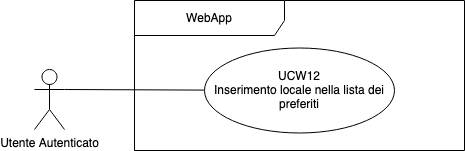
\includegraphics[scale=0.5]{UC_images/UCW12.png} 
    \caption{UCW12 - Inserimento locale nella lista dei preferiti}
\end{figure}
\begin{itemize}
    \item \textbf{Descrizione}: L'utente autenticato inserisce un locale nella lista dei preferiti.
    \item \textbf{Attore primario}: Utente autenticato.
    \item \textbf{Precondizione}: L'utente è autenticato e si trova all’interno della piattaforma Sweeat.
    \item \textbf{Postcondizione}: Viene inserito il locale scelto dall’utente nella lista dei locali preferiti.
    \item \textbf{Scenario principale}: L’utente seleziona dalla lista dei locali il locale da inserire nella lista dei locali preferiti, cliccando su “Aggiungi ai Preferiti”.
\end{itemize}

	
	\subsection{UCW13 - Rimozione locale dalla lista dei preferiti}
	%\subsection{UCW13 - Rimozione locale dalla lista dei preferiti}
\begin{figure}[!h]
\centering
    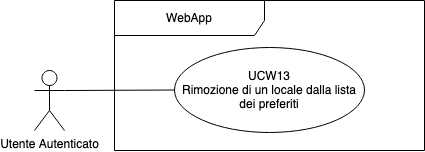
\includegraphics[scale=0.5]{UC_images/UCW13.png} 
    \caption{UCW13 - Rimozione locale dalla lista dei preferiti}
\end{figure}
\begin{itemize}
	\item \textbf{Descrizione}: L'utente autenticato rimuove un locale nella lista dei preferiti.
    \item \textbf{Attore primario}: Utente autenticato.
    \item \textbf{Precondizione}:  L’utente è autenticato nel sistema e c'è almeno un locale inserito nella lista dei locali preferiti dall’utente.
    \item \textbf{Postcondizione}: Viene rimosso il locale scelto dall’utente dalla lista dei locali preferiti.
    \item \textbf{Scenario principale}:
    \begin{enumerate}
        \item L’utente seleziona dalla lista dei locali preferiti il locale da rimuovere dalla lista dei locali preferiti;
        \item L’utente rimuove il locale da rimuovere dalla lista dei locali preferiti, cliccando su “Rimuovi dai Preferiti”.
    \end{enumerate}
\end{itemize}


	\subsection{UCE1 - Visualizza errore in caso venga inserita una stringa vuota nel nome durante la registrazione}
	%\subsection{UCE1 - Visualizza errore in caso venga inserita una stringa vuota nel nome durante la registrazione}
\begin{itemize}
\item \textbf{Descrizione}: L'utente non autenticato inserisce una stringa vuota al posto del nome in fase di registrazione alla piattaforma Sweeat.
\item \textbf{Attore primario}: Utente non autenticato.
\item \textbf{Precondizione}: L'utente inserisce una stringa vuota nel campo nome della registrazione (UCW1 §3.4.1).
\item \textbf{Postcondizione}: Viene mostrato un messaggio d'errore e l'utente non viene registrato nel sistema.

\item \textbf{Scenario principale}:
\begin{enumerate}
\item L'operazione di inserimento del nome fallisce perché viene inserita una stringa vuota;
\item Viene mostrato il corrispondente messaggio d'errore;
\item All'utente viene data la possibilità di tentare nuovamente la registrazione al sistema.
\end{enumerate}
\end{itemize}


	\subsection{UCE2 - Visualizza errore in caso venga inserita una stringa vuota nel cognome durante la registrazione}
	%\subsection{UCE2 - Visualizza errore in caso venga inserita una stringa vuota nel cognome durante la registrazione}
\begin{itemize}
\item \textbf{Descrizione}: L'utente non autenticato inserisce una stringa vuota al posto del cognome in fase di registrazione alla piattaforma Sweeat.
\item \textbf{Attore primario}: Utente non autenticato.
\item \textbf{Precondizione}: L'utente inserisce una stringa vuota nel campo cognome della registrazione (UCW1 §3.4.1).
\item \textbf{Postcondizione}: Viene mostrato un messaggio d'errore e l'utente non viene registrato nel sistema.

\item \textbf{Scenario principale}:
\begin{enumerate}
\item L'operazione di inserimento del cognome fallisce perché viene inserita una stringa vuota;
\item Viene mostrato il corrispondente messaggio d'errore;
\item All'utente viene data la possibilità di tentare nuovamente la registrazione al sistema.
\end{enumerate}
\end{itemize}	
	
	\subsection{UCE3 - Visualizza errore in caso non venga inserito un indirizzo e-mail valido durante la registrazione}
	%\subsection{UCE3 - Visualizza errore in caso non venga inserito un indirizzo e-mail valido durante la registrazione}
\begin{itemize}
\item \textbf{Descrizione}: L'utente non autenticato inserisce un indirizzo e-mail non valido in fase di registrazione alla piattaforma Sweeat.
\item \textbf{Attore primario}: Utente non autenticato.
\item \textbf{Precondizione}: L'utente inserisce un indirizzo e-mail non valido in fase di registrazione (UCW1 §3.4.1).
\item \textbf{Postcondizione}: Viene mostrato un messaggio d'errore e l'utente non viene registrato nel sistema.

\item \textbf{Scenario principale}:
\begin{enumerate}
\item L'operazione di inserimento dell'indirizzo e-mail fallisce;
\item Viene mostrato il corrispondente messaggio d'errore;
\item All'utente viene data la possibilità di tentare nuovamente la registrazione al sistema.
\end{enumerate}
\end{itemize}	
	
	\subsection{UCE4 - Visualizza errore in caso non venga inserita una password valida durante la registrazione}
	%\subsection{UCE4 - Visualizza errore in caso non venga inserita una password valida durante la registrazione}
\begin{itemize}
\item \textbf{Descrizione}: L'utente non autenticato inserisce una password non valida in fase di registrazione alla piattaforma Sweeat.
\item \textbf{Attore primario}: Utente non autenticato.
\item \textbf{Precondizione}: L'utente inserisce una password non valida in fase di registrazione (UCW1 §3.4.1).
\item \textbf{Postcondizione}: Viene mostrato un messaggio d'errore e l'utente non viene registrato nel sistema.

\item \textbf{Scenario principale}:
\begin{enumerate}
\item L'operazione di inserimento password fallisce;
\item Viene mostrato il corrispondente messaggio d'errore;
\item All'utente viene data la possibilità di tentare nuovamente la registrazione al sistema.
\end{enumerate}
\end{itemize}
	
	\subsection{UCE5 - Visualizza errore in caso non venga inserito un indirizzo e-mail esistente durante il login}
	%\subsection{UCE5 - Visualizza errore in caso non venga inserito un indirizzo e-mail esistente durante il login}
\begin{itemize}
\item \textbf{Descrizione}: L'utente non autenticato inserisce un indirizzo e-mail non registrato all'interno del sistema per accedere alla piattaforma.
\item \textbf{Attore primario}: Utente non autenticato.
\item \textbf{Precondizione}: L'utente ha inserito un indirizzo email non registrato nel sistema in fase di login (UCW2 §3.4.2).
\item \textbf{Postcondizione}: Viene mostrato un messaggio d'errore e l'utente non viene autenticato nel sistema.

\item \textbf{Scenario principale}:
\begin{enumerate}
\item L'operazione di inserimento dello username fallisce;
\item Viene mostrato il corrispondente messaggio d'errore;
\item All'utente viene data la possibilità di tentare nuovamente l'accesso al sistema.
\end{enumerate}
\end{itemize}



	\subsection{UCE6 - Visualizza errore in caso non venga inserita una password corretta durante il login}
	%\subsection{UCE6 - Visualizza errore in caso non venga inserita una password corretta durante il login}
\begin{itemize}
\item \textbf{Descrizione}: L'utente non autenticato inserisce una password non corrispondente all'indirizzo e-mail inserito per accedere alla piattaforma Sweeat.
\item \textbf{Attore primario}: Utente non autenticato.
\item \textbf{Precondizione}: L'utente inserisce una password errata in fase di login (UCW2 §3.4.2).
\item \textbf{Postcondizione}: Viene mostrato un messaggio d'errore e l'utente non viene autenticato nel sistema.

\item \textbf{Scenario principale}:
\begin{enumerate}
\item L'operazione di inserimento dello username fallisce;
\item Viene mostrato il corrispondente messaggio d'errore;
\item All'utente viene data la possibilità di tentare nuovamente l'accesso al sistema.
\end{enumerate}
\end{itemize}

	

	\subsection{UCE7 - Visualizza errore in caso non venga inserito un indirizzo e-mail esistente durante il recupero password}
	%\subsection{UCE7 - Visualizza errore in caso non venga inserito un indirizzo e-mail esistente durante il recupero password}
\begin{itemize}
\item \textbf{Descrizione}: L'utente non autenticato inserisce un indirizzo e-mail non registrato all'interno del sistema per recuperare la password con cui accedere al sistema.
\item \textbf{Attore primario}: Utente non autenticato.
\item \textbf{Precondizione}: L'utente inserisce un indirizzo e-mail non presente nel sistema durante il recupero password (UCW3 §3.4.3).
\item \textbf{Postcondizione}: Viene mostrato un messaggio d'errore e l'utente non è in grado di recuperare la password.

\item \textbf{Scenario principale}:
\begin{enumerate}
\item L'operazione di inserimento dell'indirizzo e-mail con cui l'utente è registrato alla piattaforma fallisce;
\item Viene mostrato il corrispondente messaggio d'errore;
\item All'utente viene data la possibilità di tentare nuovamente di recuperare la password con cui accedere alla piattaforma Sweeat.
\end{enumerate}
\end{itemize}
	
	\subsection{UCE8 - Visualizza errore al collegamento dell'account Instagram}
	%\subsection{UCE8 - Visualizza errore al collegamento dell'account Instagram}
\begin{itemize}
\item \textbf{Descrizione}: L'utente autenticato inserisce in maniera errata i dati di accesso al suo account Instagram.
\item \textbf{Attore primario}: Utente autenticato.
\item \textbf{Precondizione}: L'utente sta collegando il proprio account Instagram (UCW4.1 §3.5.1).
\item \textbf{Postcondizione}: Viene mostrato un messaggio d'errore e l'utente non è in grado di collegare il suo account Instagram al profilo.

\item \textbf{Scenario principale}:
\begin{enumerate}
\item L'operazione di inserimento dei dati di accesso all'account Instagram fallisce;
\item Viene mostrato il corrispondente messaggio d'errore;
\item All'utente viene data la possibilità inserire nuovamente i dati di accesso al suo account Instagram.
\end{enumerate}
\end{itemize}
	

	\subsection{UCE9 - Visualizza errore al collegamento dell'account TikTok}
	%\subsection{UCE9 - Visualizza errore al collegamento dell'account TikTok}
\begin{itemize}
\item \textbf{Descrizione}: L'utente autenticato inserisce in maniera errata i dati di accesso al suo account TikTok.
\item \textbf{Attore primario}: Utente autenticato.
\item \textbf{Precondizione}: L'utente sta collegando il proprio account TikTok (UCW4.2 §3.5.2).
\item \textbf{Postcondizione}: Viene mostrato un messaggio d'errore e l'utente non è in grado di collegare il suo account TikTok al profilo.

\item \textbf{Scenario principale}:
\begin{enumerate}
\item L'operazione di inserimento dei dati di accesso all'account Instagram fallisce;
\item Viene mostrato il corrispondente messaggio d'errore;
\item All'utente viene data la possibilità inserire nuovamente i dati di accesso al suo account TikTok.
\end{enumerate}
\end{itemize}			
	
	\subsection{UCE10 - Visualizza errore se il profilo non è esistente}
	%\subsection{UCE10 - Visualizza errore se il profilo non è esistente}
\begin{itemize}
	\item \textbf{Descrizione}: L'utente autenticato ha suggerito un profilo che non esiste su Instagram o TikTok.
    \item \textbf{Attore primario}: Utente autenticato.
    \item \textbf{Precondizione}: L’utente ha richiesto l’aggiunta di un profilo social (UCW5 §3.6, UCW6 §3.7) fornendo uno username non esistente.
    \item \textbf{Postcondizione}: Viene visualizzato un messaggio di errore e lo username non viene aggiunto al sistema.
    \item \textbf{Scenario principale}: 
    \begin{enumerate}
        \item L'inserimento dello username nella lista fallisce;
        \item Viene visualizzato a schermo un messaggio di errore il quale informa l'utente del fatto che il profilo inserito non è esistente;
        \item Viene fornita all'utente la possibilità di modificare lo username inserito.
    \end{enumerate}
\end{itemize}


	
	\subsection{UCE11 - Visualizza errore se il profilo è privato}
	%\subsection{UCE11 - Visualizza errore se il profilo è privato}
\begin{itemize}
	\item \textbf{Descrizione}: L'utente autenticato ha suggerito un profilo da aggiungere a sistema con profilo privato.
    \item \textbf{Attore primario}: Utente autenticato.
    \item \textbf{Precondizione}: L’utente ha richiesto l’aggiunta di un profilo social (UCW5 §3.6, UCW6 §3.7) fornendo lo username di un profilo privato.
    \item \textbf{Postcondizione}: Viene visualizzato un messaggio di errore e lo username non viene aggiunto al sistema.
    \item \textbf{Scenario principale}: 
    \begin{enumerate}
        \item L'inserimento dello username nella lista fallisce;
        \item Viene visualizzato a schermo un messaggio di errore il quale informa l'utente del fatto che non è possiibile inserire profili privati.
    \end{enumerate}
\end{itemize}


	
	\subsection{UCE12 - Visualizza errore se il profilo è già presente nel sistema}
	%\subsection{UCE12 - Visualizza errore se il profilo è già presente nel sistema}
\begin{itemize}
	\item \textbf{Descrizione}: L'utente autenticato ha suggerito un profilo già presente nel sistema.
    \item \textbf{Attore primario}: Utente autenticato.
    \item \textbf{Precondizione}: L’utente ha richiesto l’aggiunta di un profilo social (UCW5 §3.6, UCW6 §3.7) fornendo uno username già presente nel sistema.
    \item \textbf{Postcondizione}: Viene visualizzato un messaggio di errore e lo username non viene aggiunto al sistema.
    \item \textbf{Scenario principale}: 
    \begin{enumerate}
        \item L'inserimento dello username nella lista fallisce;
        \item Viene visualizzato a schermo un messaggio di errore il quale informa l'utente del fatto che il profilo inserito è già presente nel sistema.
    \end{enumerate}
\end{itemize}
%\clearpage 
	
	\subsection{UCE13 - Visualizza errore nei filtri}
	\subsection{UCE13 - Visualizza errore nei filtri}
\begin{itemize}
    \item \textbf{Attore primario}: Utente generico.
    \item \textbf{Precondizione}: L'utente ha inserito filtri ai quali non corrisponde alcun locale presente nel sistema.
    \item \textbf{Postcondizione}: Viene visualizzato un messaggio di errore.
    \item \textbf{Scenario principale}: 
    \begin{enumerate}
        \item L'utente inserisce dei filtri alla classifica;
        \item Nessun locale rientra nei filtri inseriti;
        \item Viene visualizzato a schermo un messaggio che informa l'utente del fatto che nessun locale rientra nei filtri inseriti.
    \end{enumerate}
\end{itemize}
	
	\subsection{UCE14 - Visualizza errore nella ricerca}
	\subsubsection{UCE14 - Visualizza errore nella ricerca}
\begin{itemize}
\item \textbf{Descrizione}:
\item \textbf{Attore primario}: Utente Generico.
\item \textbf{Precondizione}: L'utente si trova all’interno della piattaforma Sweeat e ha effettuato una ricerca di un locale.
\item \textbf{Postcondizione}: Viene mostrato un messaggio d'errore e l'utente non è in grado di visualizzare il locale cercato.
\item \textbf{Scenario principale}:
\begin{enumerate}    
	\item Il testo inserito non corrisponde ad alcun locale presenti nel database;
	\item L'operazione di ricerca del locale desiderato fallisce;
	\item Viene mostrato il corrispondente messaggio d'errore;
	\item All'utente viene data la possibilità cercare nuovamente il locale desiderato.
\end{enumerate}
\end{itemize}
	
	\subsection{UCE15 - Visualizza errore in caso non venga modificata correttamente la password}
	%\subsection{UCE15 - Visualizza errore in caso non venga modificata correttamente la password}
\begin{itemize}
\item \textbf{Descrizione}: L'utente autenticato inserisce una password non valida per accedere alla piattaforma Sweeat.
\item \textbf{Attore primario}: Utente autenticato.
\item \textbf{Precondizione}: L'utente è autenticato presso il sistema e decide di modificare la password di accesso al sistema (UCW4.3 §3.5.3).
\item \textbf{Postcondizione}: Viene mostrato un messaggio d'errore e l'utente deve inserire una nuova password per modificare la vecchia password con cui accedere alla piattaforma.

\item \textbf{Scenario principale}:
\begin{enumerate}
\item L'operazione di inserimento della password fallisce;
\item Viene mostrato il corrispondente messaggio d'errore;
\item All'utente viene data la possibilità di inserire una nuova password con cui effettuare l'accesso alla piattaforma.
\end{enumerate}
\end{itemize}

	\newpage	
	
	\section{Requisiti}
	\section{Requisiti}

\subsection{Introduzione}
In base a quanto definito nel documento \textit{\NdP}, nella sezione §2.2.3.4, il team DreamTeam ha classificato ed assegnato i requisiti come espresso nelle prossime righe.


	
	\subsection{Requisiti Funzionali}
	\subsection{Requisiti Funzionali}

\definecolor{darkblue}{cmyk}{99, 99, 0, 71}

\renewcommand{\arraystretch}{1.5}
\rowcolors{2}{gray!25}{white}
\begin{longtable}{ m{0.15\textwidth}<{\centering}  m{0.4\textwidth}<{\centering}  m{0.16\textwidth}<{\centering}  m{0.19\textwidth}<{\centering}}
	\rowcolor{darkblue}
	\textcolor{white}{\textbf{Requisito}} &\textcolor{white}{\textbf{Descrizione}}& \textcolor{white}{\textbf{Classificazione}} & \textcolor{white}{\textbf{Fonti}}\\ 

	R1FW1 & L’utente deve riuscire ad inserire i propri dati personali (nome, cognome, indirizzo e-mail e password) per effettuare la registrazione & \Ob & UCW1 \\	
	 
	R1FW2 & L’utente deve riuscire ad inserire i propri dati (indirizzo e-mail e password) per effettuare il login & \Ob & UCW2\\	

	R1FW3 & L’utente deve riuscire a recuperare la password, nel caso l’avesse dimenticata & \De & UCW3\\	
	 
	R1FE1 & All’utente viene mostrato un errore nel caso non inserisca correttamente il nome in fase di registrazione & \Ob & UCE1\\	
	 
 	R1FE2 & All’utente viene mostrato un errore nel caso non inserisca correttamente il cognome in fase di registrazione & \Ob & UCE2\\	
	 
	R1FE3 & All’utente viene mostrato un errore nel caso non inserisca correttamente l’indirizzo e-mail in fase di registrazione & \Ob & UCE3\\	

	R1FE4 & All’utente viene mostrato un errore nel caso non inserisca una password corretta in fase di registrazione & \Ob & UCE4\\	
	
	R1FE5 & All'utente viene mostrato un errore nel caso non inserisca correttamente l'indirizzo e-mail al login & \Ob & UCE5 \\
	 
	R1FE6 & All'utente viene mostrato un errore nel caso non inserisca correttamente la password al login & \Ob & UCE6 \\	 
	 
	R1FE7 & All’utente viene mostrato un errore nel caso non inserisca correttamente l’indirizzo e-mail nel recupero password & \Ob & UCE7\\	

	R1FW4 &	Un utente autenticato può accedere alla sua Area Personale & \Ob & UCW4 \\ 
	 
	R2FW4.1 & L’utente autenticato può collegare il proprio profilo Instagram  & \Ob & UCW4.1\\	
	 
	R2FE8 & All’utente autenticato viene mostrato un messaggio d’errore nel caso il collegamento al profilo Instagram non vada a buon fine & \Ob & UCE8\\	
	 
	R2FW4.2 & L’utente autenticato può collegare al proprio profilo l’account TikTok & \Ob & UCW4.2\\		 

	R2FE9 & All’utente autenticato viene mostrato un messaggio d’errore nel caso il collegamento al profilo TikTok non vada a buon fine  & \Ob & UCE9 \\		
	 
	R3FW4.3 & L’utente autenticato può modificare la password con cui accede al sistema & \Fa & UCW4.3\\				
	 
	R3FE15 & All’utente autenticato viene mostrato un errore nel caso non inserisca una password valida, in fase di modifica  & \Fa & UCE15\\			
	  	 	 	
	R1FW5 & L’utente autenticato può suggerire dei profili social da cui fare il crawling dei dati & \Ob & UCW5, UCW6\\		
	 
	R2FE10 & All’utente autenticato viene mostrato un messaggio d’errore nel caso suggerisca un profilo social inesistente & \De & UCE10\\		

	R2FE11 & All’utente autenticato viene mostrato un messaggio d’errore nel caso l’utente suggerito abbia un profilo privato & \De & UCE11\\
	 
	R2FE12 & All’utente autenticato viene mostrato un messaggio d’errore nel caso suggerisca un profilo già presente a sistema & \De & UCE12\\			
	 
	R1FW7 & L’utente può visualizzare la classifica con i locali presenti nel database della piattaforma & \Ob & UCW7\\	
	 
	R1FW8 & L’utente può filtrare la classifica & \Ob & UCW8\\		
	
	R2FE13 & Nel caso non ci sia alcun risultato compatibile con i filtri applicati, viene mostrato un errore & \De & UCE13\\	
	 
	R1FW8.1 & L’utente può filtrare la classifica dei locali presenti nel database del sistema in base alla zona & \Ob & UCW8.1\\	
	 
	R2FW8.2 & L’utente può filtrare la classifica dei locali presenti nel database del sistema per giorno ed orario di apertura & \De & UCW8.2\\	
	 
	R2FW8.3 & L’utente può filtrare la classifica dei locali presenti nel database del sistema in base al tipo di cucina & \De & UCW8.3\\	
	 
	R2FW8.4 & L’utente può filtrare la classifica dei locali presenti nel database del sistema per fascia di prezzo & \De & UCW8.4\\	 
	 
	R1FW8.5 & L’utente può filtrare la classifica dei locali presenti nel database del sistema in base al punteggio & \Ob & UCW8.5\\	 
	 
	R3FW9 & L’utente può modificare l’ordinamento di visualizzazione della classifica & \Fa & UCW9\\	
	 
	R3FW9.1 & L’utente può modificare la visualizzazione dei risultati della classifica, impostando il peso dei social & \Fa & UCW9.1\\	 
	 
	R3FW9.2 & L’utente può modificare la visualizzazione dei risultati della classifica, impostando il peso dei tipi di contenuto & \Fa & UCW9.2\\	  
	 
	R1FW10 & L’utente può cercare un locale presente nel database del sistema tramite il suo nome & \Ob & UCW10 \\	 
	 
	R2FE14 & All’utente viene mostrato un errore in caso il locale cercato non sia presente nel sistema & \De & UCE14\\	 
	 	 
	R1FW11 & L’utente può visualizzare le informazioni di un locale presente nel sistema & \Ob & UCW11\\	 	 	 	

	R2FW12 & L’utente può aggiungere un locale alla lista dei preferiti & \De &  UCW12\\

	R2FW13 & L’utente può rimuovere un locale dalla lista dei preferiti & \De & UCW13\\

	R3F1 & L’utente può suggerire delle modifiche da apportare relative alle informazioni di un locale & \Fa & \Di \\

	\hiderowcolors \caption{Requisiti Funzionali}
\end{longtable}

\clearpage
	
	\subsection{Requisiti di Qualità}
	\subsection{Requisiti di Qualità}

\definecolor{darkblue}{cmyk}{99, 99, 0, 71}

\renewcommand{\arraystretch}{1.5}
\rowcolors{2}{gray!25}{white}
\begin{longtable}{ m{0.15\textwidth}<{\centering}  m{0.4\textwidth}<{\centering}  m{0.16\textwidth}<{\centering}  m{0.19\textwidth}<{\centering}}
	\rowcolor{darkblue}
	\textcolor{white}{\textbf{Requisito}} &\textcolor{white}{\textbf{Descrizione}}& \textcolor{white}{\textbf{Classificazione}} & \textcolor{white}{\textbf{Fonti}}\\ 

	R1Q1 & Il sistema dovrà essere sviluppato secondo quanto espresso nel documento \textit{\NdP} & \Ob & \Di \\
	
	R1Q2 & Deve essere fornito un documento di sintesi in lingua italiana sui limiti dei social utilizzati & \Ob & \Ca \\
	
	R1Q3 & Deve essere fornita una documentazione dettagliata in lingua italiana di tutte le API\textsuperscript{G} & \Ob & \Ca \\

	R1Q4 & Deve essere fornito un documento in lingua italiana realtivo ai limiti di servizi e algoritmi usati per estrarre la valutazione di un luogo di interesse & \Ob & \Ca \\

	R1Q5 & Il codice sorgente della piattaforma sarà reperibile su \textit{GitHub} & \Ob & VerbaleInterno-2021.11.29 \\
	
	R1Q6 & Dovrà essere realizzato un manuale interno in lingua italiana  & \Ob & \Di \\

	\hiderowcolors \caption{Requisiti di Qualità}
\end{longtable}

\clearpage
	
	\subsection{Requisiti di Vincolo}
	\subsection{Requisiti di Vincolo}

\definecolor{darkblue}{cmyk}{99, 99, 0, 71}

\renewcommand{\arraystretch}{1.5}
\rowcolors{2}{gray!25}{white}
\begin{longtable}{ m{0.15\textwidth}<{\centering}  m{0.4\textwidth}<{\centering}  m{0.16\textwidth}<{\centering}  m{0.19\textwidth}<{\centering}}
	\rowcolor{darkblue}
	\textcolor{white}{\textbf{Requisito}} &\textcolor{white}{\textbf{Descrizione}}& \textcolor{white}{\textbf{Classificazione}} & \textcolor{white}{\textbf{Fonti}}\\ 

	R1V1 & L’interfaccia utente del sistema dovrà essere sviluppato sfruttando il framework React & \Ob & \Vi{} 2022-01-13 \\	

	R1V2 & Il sistema dovrà funzionare sul browser Chrome dalla versione più recente (97.0.4692) & \Ob & \Ve{} 2022-01-26 \\	
	 
	R1V3 & Il sistema dovrà funzionare sul browser Microsoft Edge dalla versione più recente (96.0.1031.0) & \Ob & \Ve{} 2022-01-26 \\	

	R1V4 & Il sistema dovrà funzionare sul browser Firefox dalla versione più recente (96.0.2) & \Ob & \Ve{} 2022-01-26 \\	
	 
	R1V5 & Il sistema dovrà funzionare sul browser Safari dalla versione più recente (15.3) & \Ob & \Ve{} 2022-01-26 \\	
	 
	R1V6 & Il sistema dovrà sfruttare i servizi offerti da AWS\textsuperscript{G} & \Ob & \Ca \\	
	 
	R2V1 & Il sistema dovrà sfruttare il database Amazon Aurora Serverless\textsuperscript{G} & \De & \Vi{} 2022-01-13 \\
	
	R1V7 & Il sistema dovrà sfruttare il servizio di calcolo AWS Lambda\textsuperscript{G} & \Ob & \Ca \\	
	 
	R1V8 & Il sistema dovrà sfruttare il servizio AWS API Gateway\textsuperscript{G} & \Ob & \Ca \\
	
	R1V9 & Il sistema dovrà sfruttare il servizio Amazon Rekognition\textsuperscript{G} & \Ob & \Ca \\
		
	R1V10 & Il sistema dovrà sfruttare il servizio Amazon Comprehend\textsuperscript{G} & \Ob & \Ca \\	 

	R2V2 & Le API per lo sviluppo del crawler Instagram dovranno essere sviluppate in Python & \De & \Vi{} 2022-01-13 \\	
	 
	R2V3 & Le API per lo sviluppo del crawler TikTok dovranno essere sviluppate in Python & \De & \Vi{} 2022-01-13 \\	
	 
	R1V11 & È necessario sfruttare un’architettura a microservizi\textsuperscript{G}  & \Ob & \Ca \\	
	 
	R1V12 & È necessario non superare la soglia di 2000\$ di credito per i servizi offerti da AWS & \Ob & \Ve{} 2022-01-26 \\	
	
	\hiderowcolors \caption{Requisiti di Vincolo}
\end{longtable}

\pagebreak
	
	\subsection{Requisiti Prestazionali}
	\subsection{Requisiti Prestazionali}

Non sono stati individuati requisiti prestazionali per quanto riguarda i requisiti obbligatori. I servizi di AWS utilizzati per realizzare la piattaforma non presentano problemi a livello di performance. 	
	
	\subsection{Tracciamento}
	\subsection{Tracciamento}

\subsubsection{Fonte - Requisiti}

\definecolor{darkblue}{cmyk}{99, 99, 0, 71}

\begin{table}[!htbp]
\rowcolors{2}{gray!25}{white}
\renewcommand{\arraystretch}{1.5}
\begin{tabular}{ m{0.3\textwidth}<{\centering}  m{0.65\textwidth}<{\centering} }
	\rowcolor{darkblue}
	\textcolor{white}{\textbf{Fonte}} &\textcolor{white}{\textbf{Requisiti}}\\ 

	Capitolato & R1Q2, R1Q3, R1Q4, R1V6, R1V7, R1V8, R1V9, R1V10, R1V11\\	

	Decisione Interna & R3F1, R1Q1, R1Q6 \\
	
	\Vi{} 2022-01-13 & R1V1, R2V1, R2V2, R2V3 \\
	
	\Vi{} 2021-11-29 & R1Q5 \\
	
	\Ve{} 2022-01-26 & R1V2, R1V3, R1V4, R1V5, R1V12 \\

\end{tabular}
\caption{Tabella di tracciamento Fonte - Requisiti (1)}
\end{table}

\pagebreak
\subsubsection{Fonte - Requisiti}

\begin{table}[!htbp]
\rowcolors{2}{gray!25}{white}
\renewcommand{\arraystretch}{1.5}
\begin{tabular}{ m{0.15\textwidth}<{\centering}  m{0.3\textwidth}<{\centering} }
	\rowcolor{darkblue}
	\textcolor{white}{\textbf{Fonte}} &\textcolor{white}{\textbf{Requisiti}}\\ 

	UCW1 & R1FW1\\	
	 
	UCW2 & R1FW2\\	

	UCW3 & R1FW3\\	
	 
	UCE1 & R1FE1\\	
	 
	UCE2 & R1FE2\\	
	 
	UCE3 & R1FE3\\	

	UCE4 & R1FE4\\	
	
	UCE5 & R1FE5\\
	 
	UCE6 & R1FE6\\	 
	 
	UCE7 & R1FE7\\	

	UCW4 & R1FW4\\ 
	 
	UCW4.1 & R1FW4.1\\	
	 
	UCE8 & R1FE8 \\	
	 
	UCW4.2 & R1FW4.2\\		 

	UCE9 & R1FE9\\		
	 
	UCW4.3 & R3FW4.3 \\				
	 
	UCE15 & R3FE15\\			
	  	 	 	
	UCW5 & R1FW5\\		
	 
	UCW6 & R1FW5 \\
	
	UCE10 & R2FE10 \\

\end{tabular}
\begin{tabular}{ m{0.15\textwidth}<{\centering}  m{0.3\textwidth}<{\centering} }
	\rowcolor{darkblue}
	\textcolor{white}{\textbf{Fonte}} &\textcolor{white}{\textbf{Requisiti}}\\ 

	UCE11 & R2FE11\\
	 
	UCE12 & R2FE12 \\			
	 
	UCW7 & R1FW7 \\	
	 
	UCW8 & R1FW8 \\		
	
	UCE13 & R2FE13  \\	
	 
	UCW8.1 & R1FW8.1 \\	
	 
	UCW8.2 & R2FW8.2 \\	
	 
	UCW8.3 & R2FW8.3\\	
	 
	UCW8.4 & R2FW8.4 \\	 
	 
	UCW8.5 & R1FW8.5 \\	 
	 
	UCW9 & R3FW9 \\	
	 
	UCW9.1 & R3FW9.1\\	 
	 
	UCW9.2 & R3FW9.2\\	  
	 
	UCW10 & R1FW10 \\	 
	 
	UCE14 & R2FE14\\	 
	 	 
	UCW11 & R1FW11\\	 	 	 	

	UCW12 & R2FW12\\

	UCW13 & R2FW13 \\

	R1FW1 & UCW1 \\

\end{tabular}
\caption{Tabella di tracciamento Fonte - Requisiti (2)}
\end{table}

\pagebreak

\subsubsection{Requisito - Fonti}

\begin{table}[!htbp]
\rowcolors{2}{gray!25}{white}
\renewcommand{\arraystretch}{1.5}
\begin{tabular}{ m{0.125\textwidth}<{\centering}  m{0.15\textwidth}<{\centering} }
	\rowcolor{darkblue}
	\textcolor{white}{\textbf{Requisito}} &\textcolor{white}{\textbf{Fonti}}\\ 	
	 
	R1FW2 & UCW2\\	

	R1FW3 & UCW3\\	
	 
	R1FE1 & UCE1\\	
	 
 	R1FE2 & UCE2\\	
	 
	R1FE3 & UCE3\\	

	R1FE4 & UCE4\\	
	
	R1FE5 & UCE5 \\
	 
	R1FE6 & UCE6 \\	 
	 
	R1FE7 & UCE7\\	

	R1FW4 & UCW4 \\ 
	 
	R1FW4.1 & UCW4.1\\	
	 
	R1FE8 & UCE8\\	
	 
	R1FW4.2 & UCW4.2\\		 

	R1FE9 & UCE9 \\		
	 
	R3FW4.3 & UCW4.3\\				
	 
	R3FE15 & UCE15\\			
	  	 	 	
	R1FW5 & UCW5, UCW6\\		
	 
	R2FE10 & UCE10\\
	
	R2FE11 & UCE11\\
	 
	R2FE12 & UCE12\\	
	
	R1FW7 & UCW7\\

\end{tabular}
\begin{tabular}{ m{0.125\textwidth}<{\centering}  m{0.15\textwidth}<{\centering} }
	\rowcolor{darkblue}
	\textcolor{white}{\textbf{Requisito}} &\textcolor{white}{\textbf{Fonti}}\\ 			 
	 
	R1FW8 & UCW8\\		
	
	R2FE13 & UCE13\\	
	 
	R1FW8.1 & UCW8.1\\	
	 
	R2FW8.2 & UCW8.2\\	
	 
	R2FW8.3 & UCW8.3\\	
	 
	R2FW8.4 & UCW8.4\\	 
	 
	R1FW8.5 & UCW8.5\\	 
	 
	R3FW9 & UCW9\\	
	 
	R3FW9.1 & UCW9.1\\	 
	 
	R3FW9.2 & UCW9.2\\	  
	 
	R1FW10 & UCW10 \\	 
	 
	R2FE14 & UCE14\\	 
	 	 
	R1FW11 & UCW11\\	 	 	 	

	R2FW12 & UCW12\\

	R2FW13 & UCW13\\

	R3F1 & \Di \\
	
	R1Q1 & \Di \\
	
	R1Q2 & \Ca \\
	
	R1Q3 & \Ca \\
	
	R1Q4 &  \Ca \\
	
	R1Q5 & \Vi{} 2021-11-29\\
	
\end{tabular}
\begin{tabular}{ m{0.125\textwidth}<{\centering}  m{0.15\textwidth}<{\centering} }
	\rowcolor{darkblue}
	\textcolor{white}{\textbf{Requisito}} &\textcolor{white}{\textbf{Fonti}}\\ 

	R1Q6 & \Di \\

	R1V1 & \Vi{} 2022-01-13 \\	

	R1V2 & \Ve{} 2022-01-26 \\	
	 
	R1V3 & \Ve{} 2022-01-26 \\	

	R1V4 & \Ve{} 2022-01-26 \\	
	 
	R1V5 & \Ve{} 2022-01-26 \\	
	 
	R1V6 & \Ca \\	
	 
	R2V1 & \Vi{} 2022-01-13 \\
	
	R1V7 & \Ca \\	
	 
	R1V8 & \Ca \\	 
	
	R1V9 & \Ca \\	
	
	R1V10 & \Ca \\
	
	R1V11 & \Ca \\

	R2V2 & \Vi{} 2022-01-13 \\	
	 
	R2V3 & \Vi{} 2022-01-13 \\	
	 
	R1V12 & \Ve{} 2022-01-26 \\	

\end{tabular}
\caption{Tabella di tracciamento Requisito - Fonti}
\end{table}

\subsubsection{Riepilogo Requisiti}

\begin{table}[!htbp]
\rowcolors{2}{gray!25}{white}
\renewcommand{\arraystretch}{1.5}
\begin{tabular}{ m{0.175\textwidth}<{\centering}  m{0.175\textwidth}<{\centering}  m{0.175\textwidth}<{\centering}  m{0.175\textwidth}<{\centering}  m{0.175\textwidth}<{\centering} }
	\rowcolor{darkblue}
	\textcolor{white}{\textbf{Tipologia}} &\textcolor{white}{\textbf{\Ob}}& \textcolor{white}{\textbf{\De}} & \textcolor{white}{\textbf{\Fa}}&\textcolor{white}{\textbf{Totale}}\\ 
	Funzionale & 21 & 11 & 6 & 38\\	
	Qualità & 6 & 0 & 0 & 6 \\	
	Vincolo & 12 & 3 & 0 & 15 \\	
	\textbf{Totale} & 39 & 	14 & 6 & 59
\end{tabular}
\caption{Riepilogo dei Requisiti}
\end{table}	
	\newpage

	\section{Limiti dei social utilizzati}
	%\section{Limiti dei social utilizzati}
Come richiesto dal proponente, il team dovrà realizzare un'analisi sui limiti dei social utilizzati al fine di capire la realizzabilità di determinati requisiti.

\subsection{Instagram}
\subsubsection{Limiti}
Durante lo sviluppo, il team ha riscontrato alcuni problemi che evidenziano i limiti nell'utilizzo di un crawler su Instagram.
\begin{itemize}
    \item Per effettuare crawling, è necessario utilizzare un account instagram;
    \item Effettuare troppe richieste in poco tempo porta ad alcuni warning che impediscono l'esecuzione del programma;
    \item A seguito dei warning, Instagram può chiedere di inserire un codice di conferma ricevuto via email per poter continuare ad utilizzare l'account con cui si sta facendo crawling. Questo comporta l'intervento di una persona per sbloccare l'account;
    \item Il susseguirsi degli eventi escritti ai punti precedenti porta al ban definitivo dell'account Instagram;
    \item Dato che gli indirizzi IP di aws sono in gran parte presenti nella black-list di Instagram, effettuare le operazioni di crawling da una aws lambda è quasi impossibile perché porta al ban dell'account in tempi brevissimi.
\end{itemize}

\subsubsection{Soluzioni}
Il team ha individuato le seguenti soluzioni ai problemi descritti in precedenza.
\begin{itemize}
    \item Creare innumerevoli account in modo da averne sempre a disposizione a seguito di un ban, gli account per funzionare a dovere dovranno essere stati creati con qualche settimana di anticipo dato che Instagram tende a bloccare più facilemnte un account appena creato;
    \item Introdurre delle sleep di un tempo random da 5 a 15 secondi tra una richiesta e l'altra, in modo da emulare il comportamento di un umano;
    \item Fare girare il crawler esclusivamente in locale data l'impossibilità di farlo su una aws lambda (sarebbe possibile effettuare il crawling su una aws lambda, ma solo utilizzando dei proxy domestici che il team non ha avuto a disposizione);
    \item Provare ad utilizzare una VPN per effettuare il crawling, soluzione che ha non ha avuto l'effetto desiderato, ma che ha portato al rapido ban di un account;
    \item Salvare a database i dati relativi alle location dei post in modo tale da poter fare un controllo nel database prima di effettuare un richiesta ad Instagram.
\end{itemize}

\subsubsection{Conclusioni}
Nonostante i limiti descritti ai punti precedenti, il team è riuscito a raccogliere i seguenti dati analizzando i post di 340 utenti:
\begin{itemize}
    \item più di 5000 location delle quali più della metà relative a ristoranti;
    \item più di 5000 post relativi a ristoranti;
    \item più di 13000 immagini relative a ristoranti.
\end{itemize}
I numeri ottenuti sono limitati dalle politiche anti-crawling di Instagram, ma il codice realizzato sarebbbe comunque in grado di funzionare su più ampia scala con l'aggiunta di alcune risorse come:
\begin{itemize}
    \item sostituzione delle chiamate alle API private di instagram per ottenere dettagli sul geotag di un post con le API di google maps;
    \item esecuzione parallela di più istanze del crawler, oguna con un account Instagram e un proxy domestico differente.
\end{itemize}

\subsection{TikTok}
Per quanto riguarda il crawling con TikTok, il team ha riscontrato numerosi problemi durante la fase di sviluppo del \textit{Proof of Concept}, i quali hanno portato a ritenere queste operazioni come non fattibili a causa dei seguenti motivi:
\begin{itemize}
    \item Tiktok a differenza di Instagram è molto più severo nei confronti di chi effettua crawling;
    \item L'unico crawler open source funzionante individuato dal team, dopo pochissime operazioni di crawling porta al ban dell'ip\textsuperscript{G}. Nonostante ciò il team è riuscito ad aggirare questo problema utilizzando dei proxy\textsuperscript{G} gratuiti e creando un algoritmo che testasse la validità di questi proxy;
    \item Le alternative valide al crawler utilizzato sono tutte a pagamento e quindi non utilizzabili all'interno di questo progetto;
    \item Il crawler utilizzato dal team non può funzionare all'interno di una lambda dato che fa uso del framework playwright\textsuperscript{G}, per questo problema dopo lunghe ricerche il team non è riuscito a trovare una soluzione attuabile;
    \item L'idea di creare un nostro crawler è troppo dispendiosa se messa a confronto con le ore lavorative a disposizione, dato che dopo un po' di tentativi il team si è reso conto che un semplice parser html\textsuperscript{G} non sarà sufficiente a causa dell'autenticazione (la quale necessita la risoluzione di un captcha\textsuperscript{G}) e dell'utilizzo da parte di TikTok di un sistema di signed request\textsuperscript{G};
    \item Per quanto riguarda la versione desktop di TikTok, non è possibile guardare i profili seguiti da un utente. Questo rende irrealizzabile il caso d'uso UCW6;
    \item Difficilmente si riuscirà ad associare un locale ad un post, dato che TikTok non offre la possibilità di mettere un geotag\textsuperscript{G}. Anche ricavando un indirizzo dal testo del post risulterebbe troppo oneroso associare quell'indirizzo ad uno specifico locale, infatti l'unica soluzione pensata dal team è quella di utilizzare le API di Google Maps, le quali offrono un numero di chiamate troppo piccolo nella versione gratuita;
	
	    
    \item A tutto questo si aggiunge il fatto che TikTok non viene utilizzato spesso per caricare contenuti relativi ai ristoranti, c’è quindi il rischio di impiegare molte risorse per ricavare pochissimi dati utili.
\end{itemize}
Dopo aver presentato queste considerazioni relative al rapporto costi/benefici al proponente, ci è stato comunicato che l’analisi svolta risulta sufficiente. A tal proposito,  questa eventualità era già stata presa in considerazione dal proponente stesso, il quale ha confermato al team che il prodotto finale sfrutterà solo Instagram, mentre la componente TikTok potrà essere esclusa.
	
\end{document}
